\documentclass[UTF8,a4paper]{article}
\usepackage{fancyhdr}
\usepackage{ctex}
\usepackage{CJK}
\usepackage{amsmath}
\usepackage{listings}
\usepackage{graphics}
\usepackage{graphicx}
\usepackage{color}
\usepackage{xcolor}
\usepackage{geometry}
\usepackage{indentfirst}
\setlength{\parindent}{2em}
\geometry{left=1.5cm,right=1.5cm,top=2cm,bottom=1.5cm}
\lstset{breaklines}%这条命令可以让LaTeX自动将长的代码行换行排版
\lstset{extendedchars=false}%这一条命令可以解决代码跨页时,章节标题,页眉等汉字不显示的问题
\lstset{ 
	language=Python,                % choose the language of the code
	basicstyle=\small\sf,    % the size of the fonts that are used for the code
	tabsize=3,                            % sets default tabsize to 3 spaces
	numbers=left,                   % where to put the line-numbers
	numberstyle=\tiny,              % the size of the fonts that are used for the line-numbers
	stepnumber=1,                   % the step between two line-numbers. If it's 1 each line
	% will be numbered
	numbersep=5pt,                  % how far the line-numbers are from the code   %
	keywordstyle=\color[RGB]{33,33,234},               % keywords
	commentstyle=\color[RGB]{0,0,0},    % comments
	stringstyle=\color[rgb]{0.170,0.187,0.102},      % strings
    backgroundcolor=\color{white},
    rulesepcolor=\color[RGB]{20,20,20},  % choose the background color. You must add \usepackage{color}
	showspaces=false,               % show spaces adding particular underscores
	showstringspaces=false,         % underline spaces within strings
	showtabs=false,                 % show tabs within strings adding particular underscores                frame = single,         % adds a frame around the code
	captionpos=b,                   % sets the caption-position to bottom
	breaklines=true,                % sets automatic line breaking
	breakatwhitespace=false,        % sets if automatic breaks should only happen at whitespace
	title=\lstname,                 % show the filename of files included with \lstinputlisting;
	% also try caption instead of title
	mathescape=true,escapechar=?    % escape to latex with ?..?
	escapeinside={\%*}{*)},         % if you want to add a comment within your code
	%columns=fixed,                  % nice spacing
	%morestring=[m]',                % strings
	%morekeywords={%,...},%          % if you want to add more keywords to the set
	%    break,case,catch,continue,elseif,else,end,for,function,global,%
	%    if,otherwise,persistent,return,switch,try,while,...},%
}
\pagestyle{fancy}
\lhead{数据结构实验报告}
\chead{}
\rhead{\bfseries 22920182204393庄震丰}
\lfoot{}
\cfoot{\thepage}
\rfoot{}
\renewcommand{\headrulewidth}{0.4pt}
\begin{document}
\begin{center}
    \textbf{\LARGE{数据结构上机实验报告}}\\[0.5cm]
    \normalsize{庄震丰 22920182204393}\\[0.3cm]
    \large{Jun. $9^{th}$, 2020}
\end{center}
\section{实现聊天电脑版微信}
\subsection{需求分析}
实现一个简单的聊天功能的程序。
\subsection{实现过程}
一个简单的局域网多人聊天室软件。实现局域网内的聊天室创建、搜索和加入。必须在局域网的条件下使用(暂不完全支持热点,打开热点的用户将无法使用)。
使用时要在设置中打开软件的通知权限。\\
创建聊天室:创建服务器并加入到自己的聊天室中,同时向局域网可见。\\
结构分为:Client端和server端。\\
实现语言:python\\[0.5cm]
\textbf{主要功能(用户手册)}:
\begin{itemize}
    \item 运行服务器建立连接~~ server.py
    \item 运行客户端进行登陆~~ client.py
    \item 名称更改 ~~setname~nickname
    \item 信息发送 ~~send~message
    \item 寻求帮助 ~~help~[命令名称]
    \item ...
\end{itemize}
\subsection{实现代码}
\textbf{clinet.py}
\begin{lstlisting}
    import socket
    import threading
    import json
    from cmd import Cmd
    import datetime
    
    class Client(Cmd):
        """
        客户端
        """
        prompt = ''
        intro = datetime.datetime.now().strftime('%Y-%m-%d %H:%M:%S')+'\n'+'[Welcome] 简易聊天室客户端\n' + '[Welcome] 输入help来获取帮助\n'
    
        def __init__(self):
            """
            构造
            """
            super().__init__()
            self.__socket = socket.socket(socket.AF_INET, socket.SOCK_STREAM)
            self.__id = None
            self.__nickname = None
    
        def __receive_message_thread(self):
            """
            接受消息线程
            """
            while True:
                # noinspection PyBroadException
                try:
                    buffer = self.__socket.recv(1024).decode()
                    obj = json.loads(buffer)
                    print(datetime.datetime.now().strftime('%Y-%m-%d %H:%M:%S')+'\n'+'[' + str(obj['sender_nickname']) + '(' + str(obj['sender_id']) + ')' + ']', obj['message'])
                except Exception:
                    print(datetime.datetime.now().strftime('%Y-%m-%d %H:%M:%S')+'\n'+'[Client] 无法从服务器获取数据')
    
        def __send_message_thread(self, message):
            """
            发送消息线程
            :param message: 消息内容
            """
            self.__socket.send(json.dumps({
                'type': 'broadcast',
                'sender_id': self.__id,
                'message': message
            }).encode())
    
        def start(self):
            """
            启动客户端
            """
            self.__socket.connect(('127.0.0.1', 8888))
            self.cmdloop()
    
        def do_login(self, args):
            """
            登录聊天室
            :param args: 参数
            """
            nickname = args.split(' ')[0]
    
            # 将昵称发送给服务器,获取用户id
            self.__socket.send(json.dumps({
                'type': 'login',
                'nickname': nickname
            }).encode())
            # 尝试接受数据
            # noinspection PyBroadException
            try:
                buffer = self.__socket.recv(1024).decode()
                obj = json.loads(buffer)
                if obj['id']:
                    self.__nickname = nickname
                    self.__id = obj['id']
                    print(datetime.datetime.now().strftime('%Y-%m-%d %H:%M:%S')+'\n'+'[Client] 成功登录到聊天室')
    
                    # 开启子线程用于接受数据
                    thread = threading.Thread(target=self.__receive_message_thread)
                    thread.setDaemon(True)
                    thread.start()
                else:
                    print(datetime.datetime.now().strftime('%Y-%m-%d %H:%M:%S')+'\n'+'[Client] 无法登录到聊天室')
            except Exception:
                print(datetime.datetime.now().strftime('%Y-%m-%d %H:%M:%S')+'\n'+'[Client] 无法从服务器获取数据')
    
        def do_send(self, args):
            """
            发送消息
            :param args: 参数
            """
            message = args
            # 显示自己发送的消息
            print(datetime.datetime.now().strftime('%Y-%m-%d %H:%M:%S')+'\n'+'[' + str(self.__nickname) + '(' + str(self.__id) + ')' + ']', message)
            # 开启子线程用于发送数据
            thread = threading.Thread(target=self.__send_message_thread, args=(message, ))
            thread.setDaemon(True)
            thread.start()
    
        def do_help(self, arg):
            """
            帮助
            :param arg: 参数
            """
            command = arg.split(' ')[0]
            if command == '':
                print(datetime.datetime.now().strftime('%Y-%m-%d %H:%M:%S')+'\n')
                print('[Help] login nickname - 登录到聊天室,nickname是你选择的昵称')
                print('[Help] send message - 发送消息,message是你输入的消息')
            elif command == 'login':
                print('[Help] login nickname - 登录到聊天室,nickname是你选择的昵称')
            elif command == 'send':
                print('[Help] send message - 发送消息,message是你输入的消息')
            else:
                print('[Help] 没有查询到你想要了解的指令')
    client = Client()
    client.start()
\end{lstlisting}
\textbf{server.py}
\begin{lstlisting}
    import socket
import threading
import json
import datetime

class Server:
    """
    服务器类
    """
    def __init__(self):
        """
        构造
        """
        self.__socket = socket.socket(socket.AF_INET, socket.SOCK_STREAM)
        self.__connections = list()
        self.__nicknames = list()

    def __user_thread(self, user_id):
        """
        用户子线程
        :param user_id: 用户id
        """
        connection = self.__connections[user_id]
        nickname = self.__nicknames[user_id]
        print(datetime.datetime.now().strftime('%Y-%m-%d %H:%M:%S')+'\n'+'[Server] 用户', user_id, nickname, '加入聊天室')
        self.__broadcast(message='用户 ' + str(nickname) + '(' + str(user_id) + ')' + '加入聊天室')

        # 侦听
        while True:
            # noinspection PyBroadException
            try:
                buffer = connection.recv(1024).decode()
                # 解析成json数据
                obj = json.loads(buffer)
                # 如果是广播指令
                if obj['type'] == 'broadcast':
                    self.__broadcast(obj['sender_id'], obj['message'])
                else:
                    print(datetime.datetime.now().strftime('%Y-%m-%d %H:%M:%S')+'\n'+'[Server] 无法解析json数据包:', connection.getsockname(), connection.fileno())
            except Exception:
                print(datetime.datetime.now().strftime('%Y-%m-%d %H:%M:%S')+'\n'+'[Server] 连接失效:', connection.getsockname(), connection.fileno())
                self.__connections[user_id].close()
                self.__connections[user_id] = None
                self.__nicknames[user_id] = None

    def __broadcast(self, user_id=0, message=''):
        """
        广播
        :param user_id: 用户id(0为系统)
        :param message: 广播内容
        """
        for i in range(1, len(self.__connections)):
            if user_id != i:
                self.__connections[i].send(json.dumps({
                    'sender_id': user_id,
                    'sender_nickname': self.__nicknames[user_id],
                    'message': message
                }).encode())

    def start(self):
        """
        启动服务器
        """
        # 绑定端口
        self.__socket.bind(('127.0.0.1', 8888))
        # 启用监听
        self.__socket.listen(10)
        print(datetime.datetime.now().strftime('%Y-%m-%d %H:%M:%S')+'\n'+'[Server] 服务器正在运行......')

        # 清空连接
        self.__connections.clear()
        self.__nicknames.clear()
        self.__connections.append(None)
        self.__nicknames.append('System')

        # 开始侦听
        while True:
            connection, address = self.__socket.accept()
            print(datetime.datetime.now().strftime('%Y-%m-%d %H:%M:%S')+'\n'+'[Server] 收到一个新连接', connection.getsockname(), connection.fileno())

            # 尝试接受数据
            # noinspection PyBroadException
            try:
                buffer = connection.recv(1024).decode()
                # 解析成json数据
                obj = json.loads(buffer)
                # 如果是连接指令,那么则返回一个新的用户编号,接收用户连接
                if obj['type'] == 'login':
                    self.__connections.append(connection)
                    self.__nicknames.append(obj['nickname'])
                    connection.send(json.dumps({
                        'id': len(self.__connections) - 1
                    }).encode())

                    # 开辟一个新的线程
                    thread = threading.Thread(target=self.__user_thread, args=(len(self.__connections) - 1, ))
                    thread.setDaemon(True)
                    thread.start()
                else:
                    print(datetime.datetime.now().strftime('%Y-%m-%d %H:%M:%S')+'\n'+'[Server] 无法解析json数据包:', connection.getsockname(), connection.fileno())
            except Exception:
                print(datetime.datetime.now().strftime('%Y-%m-%d %H:%M:%S')+'\n'+'[Server] 无法接受数据:', connection.getsockname(), connection.fileno())
server = Server()
server.start()
\end{lstlisting}
\subsection{实现结果}
\begin{center}
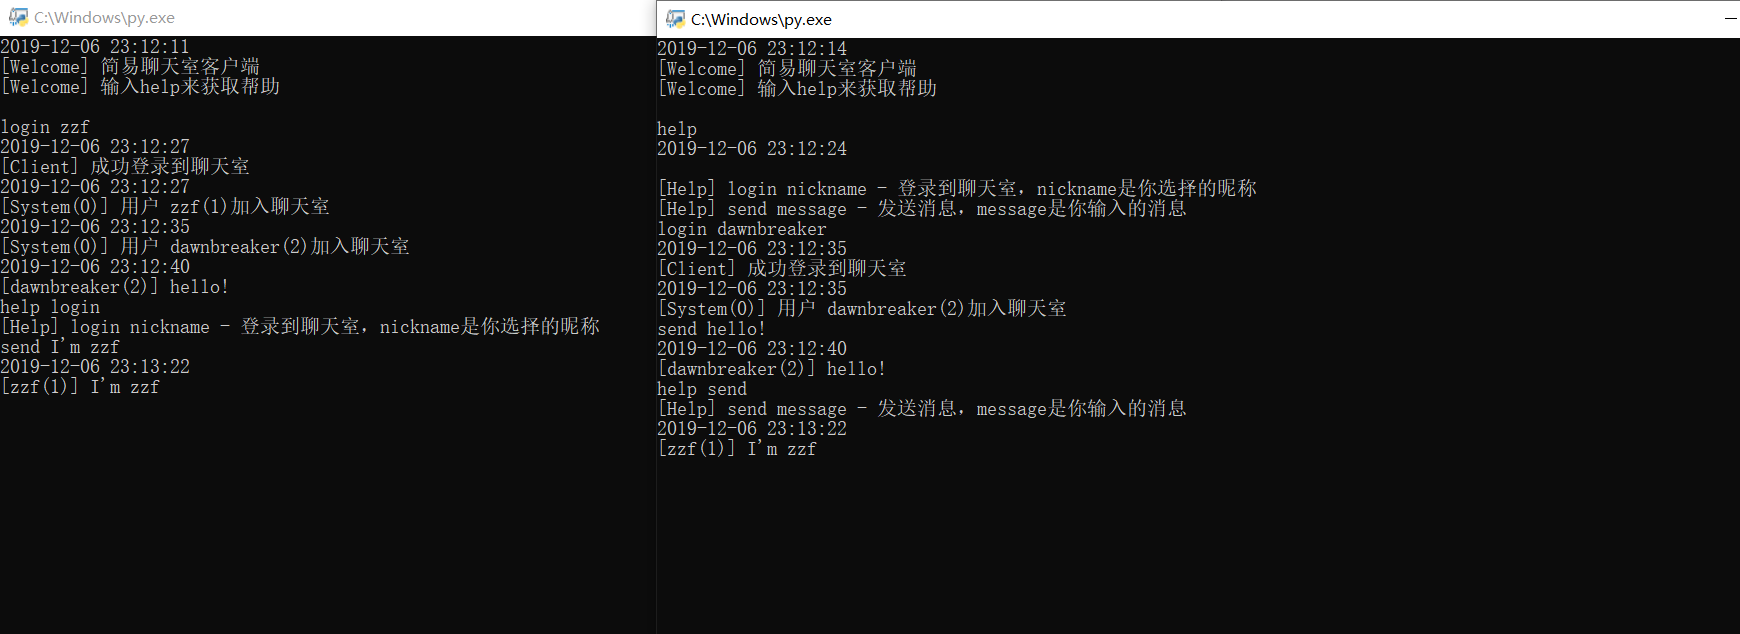
\includegraphics[scale=0.3]{chat/image/A.png}\\
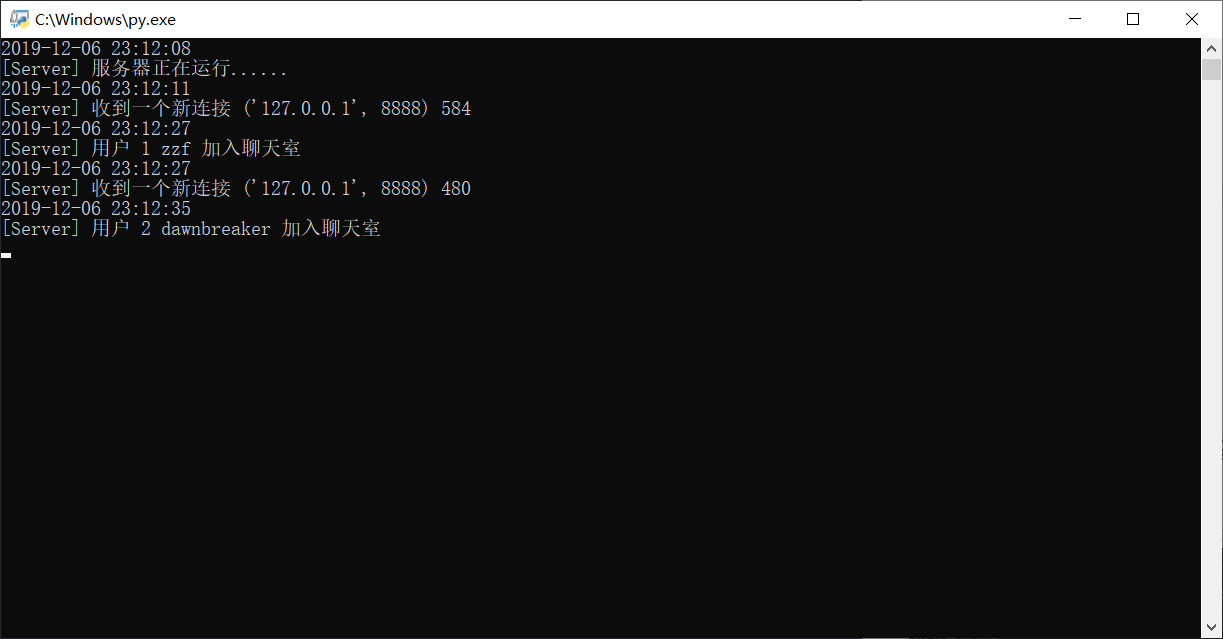
\includegraphics[scale=0.35]{chat/image/B.png}\\
\textit{图一:项目一的结果截图}\\
\end{center}
\subsection{优化总结}
\begin{itemize}
    \item 可以对窗口式的命令行进行渲染,以达到简洁易上手的App应用的目的
    \item 可以利用python的画图功能将用户进行显示
    \item 可以将python的程序应用进行打包处理,达到扩展应用的目的
\end{itemize}
\section{朋友圈关系}
\subsection{实现目的}
利用图论解决朋友圈关系的紧密程度的查询问题。
\subsection{实现过程}
利用朋友圈两两之间的关系建立点和边,针对不同的关系给予不同的边权值。紧密程度定义为:两点间的平均路径权与最短路之间的层次函数,
该函数定义为,对于此两个不同的参考因子取不同的比例,所能得到的最大值,作为两点间的关系。\\
即:
$$
f(v_i,v_j)=max_{j}  (M_{\frac{n(n-1)}{2}\times 2}\cdot P_{2\times n})
$$
其中M是:
$$
\begin{bmatrix}
    \sum w_{u_1v_1} & dis[i_1][j_1]\\
    \sum w_{u_2v_2} & dis[i_2][j_2]\\
    ... & ...
\end{bmatrix}
$$
P代表不同的权重取值,但是,p[i][1]+p[i][2]=1\\
对于不同的关系,给出了不同的亲密程度值(越小代表越亲密)\\[0.5cm]
\begin{tabular}{|c|c|c|c|c|c|c|c|c|c|c|c|c|c|c|c|}
关系类型 & mother&father&son&dauther&boyfriend&girlfriend&wife\\
\hline
权值 & 4 &4&3&3&8&8&5\\
\hline
husband&classmate&stranger&teacher&friend&boss&employee&student\\
\hline
5&15&30&16&12&23&23&16\\
\end{tabular}
\\[1cm]
关系类型到权值的映射采用了hash函数进行对应,键值为字符串,返回类型为关系对应权值。\\
并且会返回朋友圈最紧密的关系路线
\subsection{实现代码}
\begin{lstlisting}
#include<bits/stdc++.h>
#define maxn 1000
const int INF=0x3f3f3f3f;
using namespace std;
int n,m,q,ans=0,pth=INF,route=0;
int G[maxn][maxn];
bool vis[maxn][maxn];
int vrel[100];
bool rec[maxn][maxn];
string H[maxn];
void dfs(int x,int y)
{
    if (x==y) 
    {
        route=route+ans;
        if (pth>ans) 
        {
            pth=min(pth,ans);
            for (int i=1;i<=n;i++)
                for (int j=1;j<=n;j++)
                    rec[i][j]=vis[i][j];
        }
        return;
    }
    for (int i=1;i<=n;i++)
        if (G[x][i]!=INF&&!vis[x][i])
            {
                vis[x][i]=true;
                vis[i][x]=true;
                ans=ans+G[x][i];
                dfs(i,y);
                ans=ans-G[x][i];
                vis[x][i]=false;
                vis[i][x]=false;
            }
}
int Hash(string a)
{
    int key=0;
    for (int i=0;i<a.length();i++)
        key=key+a[i];
    key=key%100;
    while (H[key]!="") key=(key+1)%100;
    H[key]=a;
    return key;
}
int Index(string a)
{
    int k=0;
    for (int i=0;i<a.length();i++)
        k=k+a[i];
    k=k%100;
    while(H[k]!=a) k++;
    return k;
}
void printmap(int x)
{
    cout<<x;
    for (int i=1;i<=n;i++)
        if (rec[x][i]) 
        {
            cout<<"->";
            rec[x][i]=0;
            rec[i][x]=0;
            printmap(i);
            break;
        } 
}
void init()
{
    vrel[55]=4;
    vrel[34]=4;
    vrel[36]=3;
    vrel[49]=3;
    vrel[62]=8;
    vrel[63]=8;
    vrel[27]=5;
    vrel[41]=5;
    vrel[57]=15;
    vrel[70]=30;
    vrel[32]=16;
    vrel[33]=12;
    vrel[39]=23;
    vrel[64]=23;
    vrel[70]=16;
    for (int i=0;i<maxn;i++)
        for (int j=0;j<maxn;j++)
            {
                vis[i][j]=false;
                G[i][j]=INF;
            }
    cout<<"please input the vertex and edge number:";
    cin>>n>>m;
    for (int i=1;i<=m;i++)
    {
        int pre,aft;
        string v;
        cout<<"please add <v1,v2,relate>:";
        scanf("%d%d ",&pre,&aft);
        getline(cin,v);
        //cout<<Index(v);
        G[pre][aft]=vrel[Index(v)];
        G[aft][pre]=vrel[Index(v)];
    }
    cout<<"please input the query times:";
    cin>>q;
    for (int i=1;i<=q;i++)
    {
        int s,e;
        cout<<"start vertex and terminated vertex:";
        cin>>s>>e;
        ans=0;
        route=0;
        pth=INF;
        memset(vis,false,sizeof(vis));
        dfs(s,e);
        if (route)
        {    
            cout<<"friend distance:"<<route<<endl;
            cout<<"strongest path:"<<pth<<endl;
            printmap(s);
        }
        else cout<<"No relationship!"<<endl;
    }
}

int main()
{
    string a[15]={"mother","father","son","dauther","boyfriend","girlfriend","wife","husband","classmate","stranger","teacher","friend","boss","employee","student"};
    for (int i=0;i<15;i++)
        Hash(a[i]);
    init();
    return 0;
}
\end{lstlisting}
\subsection{设计和调试分析}
\begin{itemize}
    \item please input the vertex and edge number ~~ 输入点和边的数目\\
    \item please add <vi,vj,relate>~~输入一条边对应的关联点和关系类型\\
    \item please input the query times ~~输入查询次数\\
    \item start vertex and terminated vertex~~输入起始点和终点\\
\end{itemize}
\subsection{测试结果}
\begin{center}
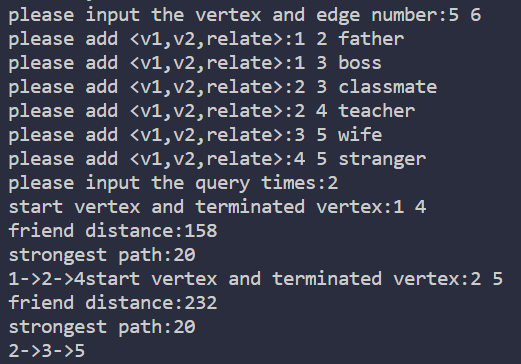
\includegraphics[scale=0.8]{friend.png}\\
\textit{图二:朋友圈关系测试结果}\\
\end{center}
如图:friend distance 代表(1,4)这一对点的边权和,最优路径权是20,给出的最优路径是1-2-4\\
对于(2,5),边权和是232,最优路径权20,最优路径为2-3-5
\newpage
\section{动态最短路}
\subsection{需求分析}
当有边权发生变化时,给出较优化的算法去基于原来的dij函数去快速求出新的询问下的最短路。\\
\subsection{概要设计}
首先容易想到改变一个边权之后重新跑一边dijkstra算法,这样当有q次改变时对应时间复杂度达到O($qn^2$)。\\
为了减少计算时间,采用的链路变化情况分为两部分,权重增大和减小。\\
当权重增大时,受用集合sub(E(e))的节点和这些节点相关的链路才会发生变化,其他的节点链路不会发送任何变化。\\
当权重减小时,sub(E(e))的节点的最短路径减少为d=w(e)-w'(e),如果节点的最短路径值发生改变,则重新选择最短路一定会经过e。
假设N为节点结合,包含所有需要更新的节点,当N的节点有一个M.v.inc代表v节点的所有入边重最小奥迪增量值的适合,L为链路集合,存储所有变化的链路,每个元素e
有一个min-inc属性,代表节点E(e)最短路径的增加值,且可为负值,当有链路需要加入集合L时,执行入队操作L,出队操作将选择L重min最小的链路,并将该链路从L中移除,利用线段树维护最小值即可。\\
算法复杂度分析:\\\\
假设有一个边的权值发生变化,Q表示最短路径变化的节点的结合,$T_p$是Q中节点的数目,参数Q和$T_p$只依赖网络拓扑结构和初始的SPT,$D_{max}$表示和一个更新节点相连的链路数目的最大值。\\
复杂度为$O(T_P^2+T_P^2D_{max})$,考虑当链路的权重发生大的变化时,执行一次将花费$O(T_P)$的时间用于线性数组的查找,并且有$T_p$次这样的迭代,当一个父亲节点更新时,有个sub(v)次子节点的更新,sub(v)<$T_p$,父亲系欸但的的更新迭代次数不超过$T_p$,则有$\sum_{v\in N}|sub(v)|=T_p$
假设一条链路的更新需要花费O(1)的时间,则所有的和更新节点关联的链路更新需要$O(T_P^2D_{max})$.所以算法的运行总时间为$O(T_P^2+T_P^2D_{max})$.
\subsection{详细设计}
\begin{lstlisting}
    #include <bits/stdc++.h>
    #define pii pair<int, int>
    #define LL long long
    #define piii pair<pii, int>
    #define ls(x) (x << 1)
    #define rs(x) ((x << 1) | 1)
    using namespace std;
    const int maxn = 200010;
    vector<piii> G[maxn];
    piii edge[maxn];
    int n;
    map<int, int> mp;
    void add(int x, int y, int z, int id) {
        G[x].push_back(make_pair(make_pair(y, z), id));
        G[y].push_back(make_pair(make_pair(x, z), id));
    }
    struct node {
        bool flag;
        LL mi, Set;
    };
    struct SegmentTree {
        int n;
        node tr[maxn * 4];
        void pushup(int o) {
            tr[o].mi = min(tr[ls(o)].mi, tr[rs(o)].mi);
        }
         
        void maintain(int o, LL val) {
            tr[o].Set = min(tr[o].Set, val);
            tr[o].mi = min(tr[o].mi, tr[o].Set);
            tr[o].flag = 1;
        }
         
        void pushdown(int o) {
            if(tr[o].flag) {
                maintain(ls(o), tr[o].Set);
                maintain(rs(o), tr[o].Set);
                tr[o].Set = 1e18;
                tr[o].flag = 0;
            }
        }
         
        void build(int o, int l, int r) {
            if(l == r) {
                tr[o].mi = 1e18;
                tr[o].flag = 0;
                tr[o].Set = 1e18;
                return;
            }
            int mid = (l + r) >> 1;
            build(ls(o), l, mid);
            build(rs(o), mid + 1, r);
            tr[o].mi = 1e18;
            tr[o].flag = 0;
            tr[o].Set = 1e18;
        }
         
        void update(int o, int l, int r, int ql, int qr, LL val) {
            if(ql > qr) return;
            if(l == 0) return;
            if(l >= ql && r <= qr) {
                maintain(o, val);
                return;
            }
            pushdown(o);
            int mid = (l + r) >> 1;
            if(ql <= mid) update(ls(o), l, mid, ql, qr, val);
            if(qr > mid) update(rs(o), mid + 1, r, ql, qr, val);
            pushup(o);
        }
         
        LL query(int o, int l, int r, int pos) {
            if(l == r && l == pos) {
                return tr[o].mi;
            }
            pushdown(o);
            int mid = (l + r) >> 1;
            if(pos <= mid) return query(ls(o), l, mid, pos);
            else return query(rs(o), mid + 1, r, pos);
        }
    };
    SegmentTree st;
    struct Dj {
        priority_queue<pair<long long, int> > q;
        pii pre[maxn];
        bool in_line[maxn], v[maxn], in_tree[maxn], is_line[maxn];
        LL dis[maxn];
        vector<int> G1[maxn];
        int f[maxn];
        vector<int> line;
        vector<LL> re;
         
        void add1(int x, int y) {
            G1[x].push_back(y);
            G1[y].push_back(x);
        }
         
        void dijkstra(int s) {
            memset(v, 0, sizeof(v));
            memset(dis, 0x3f, sizeof(dis));
            q.push(make_pair(0, s));
            dis[s] = 0;
            while(q.size()) {
                int x = q.top().second;
                q.pop();
                if(v[x]) continue;
                v[x] = 1;
                for (int i = 0; i < G[x].size(); i++) {
                    int y = G[x][i].first.first;
                    LL z = G[x][i].first.second;
                    if(v[y]) continue;
                    if(dis[y] > dis[x] + z) {
                        dis[y] = dis[x] + z;
                        pre[y] = make_pair(x, G[x][i].second);
                        q.push(make_pair(-dis[y], y));
                    }
                }
            }
        }
         
        void dfs(int x, int flag, int fa) {
            f[x] = flag;
            for (int i = 0 ; i < G1[x].size(); i++) {
                int y = G1[x][i];
                if(y == fa || is_line[y]) continue;
                dfs(y, flag, x);
            }
        }
         
        void solve(int s) {
            for (int i = 1; i <= n; i++) {
                if(i == s) continue;
                add1(i, pre[i].first);
                in_tree[pre[i].second] = 1;
            }
            for (int i = n + 1 - s; i != s; i = pre[i].first) {
                line.push_back(i);
                in_line[pre[i].second] = 1;
                is_line[i] = 1;
            }
            line.push_back(s);
            is_line[s] = 1;
            for (int i = 0; i < line.size(); i++) {
                int y = line[i];
                dfs(y, y, -1);
            }  
        }
    };
    Dj dj1, dj2;
    int main() {
        int x, y, z, m, T;
        cout<<"please input the points,edges,query numbers:";
        scanf("%d%d%d", &n, &m, &T);
        cout<<"input the order of the both points and edge value:";
        for (int i = 1; i <= m; i++) {
            scanf("%d%d%d", &x, &y, &z);
            edge[i] = make_pair(make_pair(x, y), z);
            add(x, y, z, i);
        }
        dj1.dijkstra(1), dj2.dijkstra(n);
        dj1.solve(1), dj2.solve(n);
        int cnt = 0;
        for (int i = dj1.line.size() - 1; i >= 0; i--) {
            mp[dj1.line[i]] = ++cnt;
        }
        st.build(1, 1, cnt - 1);
        for (int i = 1; i <= m; i++) {
            if(dj1.in_tree[i] && dj2.in_tree[i]) continue;
            else {
                int x = edge[i].first.first, y = edge[i].first.second;
                LL tmp = 1e18;
                int l, r;
                l = min(mp[dj1.f[x]], mp[dj2.f[y]]), r = max(mp[dj1.f[x]], mp[dj2.f[y]]);
                tmp = dj1.dis[x] + dj2.dis[y] + edge[i].second;
                if(l >= 1 && r <= cnt)
                    st.update(1, 1, cnt - 1, l, r - 1, tmp);
                swap(x, y);
                l = min(mp[dj1.f[x]], mp[dj2.f[y]]), r = max(mp[dj1.f[x]], mp[dj2.f[y]]);
                tmp = dj1.dis[x] + dj2.dis[y] + edge[i].second;
                if(l >= 1 && r <= cnt)
                    st.update(1, 1, cnt - 1, l, r - 1, tmp);
            }
        }
        int cnt_T = 0;
        while(T--) {
            cnt_T++;
            LL ans = 0;
            cout<<"change edge[x]'s value to y";
            scanf("%d%d", &x, &y);
            int l1 = edge[x].first.first, r1 = edge[x].first.second;
            if(!dj1.in_line[x]) {
                ans = dj1.dis[n];
                ans = min(ans, min(dj1.dis[l1] + dj2.dis[r1] + y, dj1.dis[r1] + dj2.dis[l1] + y));
                printf("%lld\n", ans);
            } else {
                LL ans = dj1.dis[l1] + dj2.dis[r1] + y;
                ans = min(ans, dj1.dis[r1] + dj2.dis[l1] + y);
                int now = min(mp[l1], mp[r1]);
                printf("%lld\n", min(ans, st.query(1, 1, cnt - 1, now)));
            }
        }
    }
\end{lstlisting}
\subsection{设计和调试分析及测试结果说明}
\begin{center}
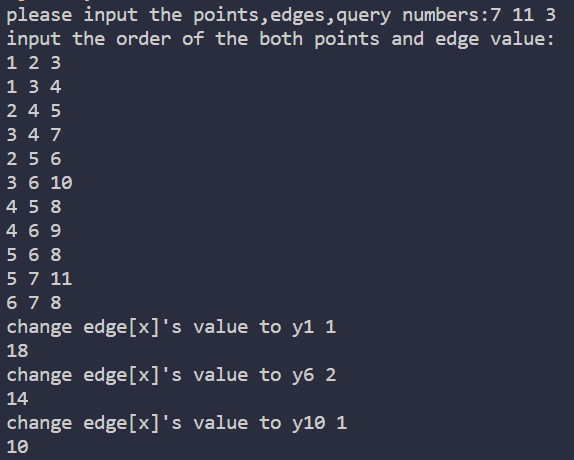
\includegraphics[scale=0.5]{dym-dijktra.png}\\
\textit{图三:动态dijkstra算法测试结果}
\end{center}
\begin{itemize}
    \item please input the points edges query numbers ~~输入图点数,边数和询问次数
    \item input the order of the both poins and edge value ~~按顺序输入边的关联点和边值
    \item change edge[x]'s value to y ~~将边x的值改为y
\end{itemize}
\textbf{测试结果说明}\\
输入的图有7个点,11条边,共有3次询问\\
第一次将第一条边的值改为1\\
第二次将第六条边的值改为2\\
第三次将第十条边的值改为1\\
得到的dij[n]分别如图所示:\\[1cm]
\begin{center}
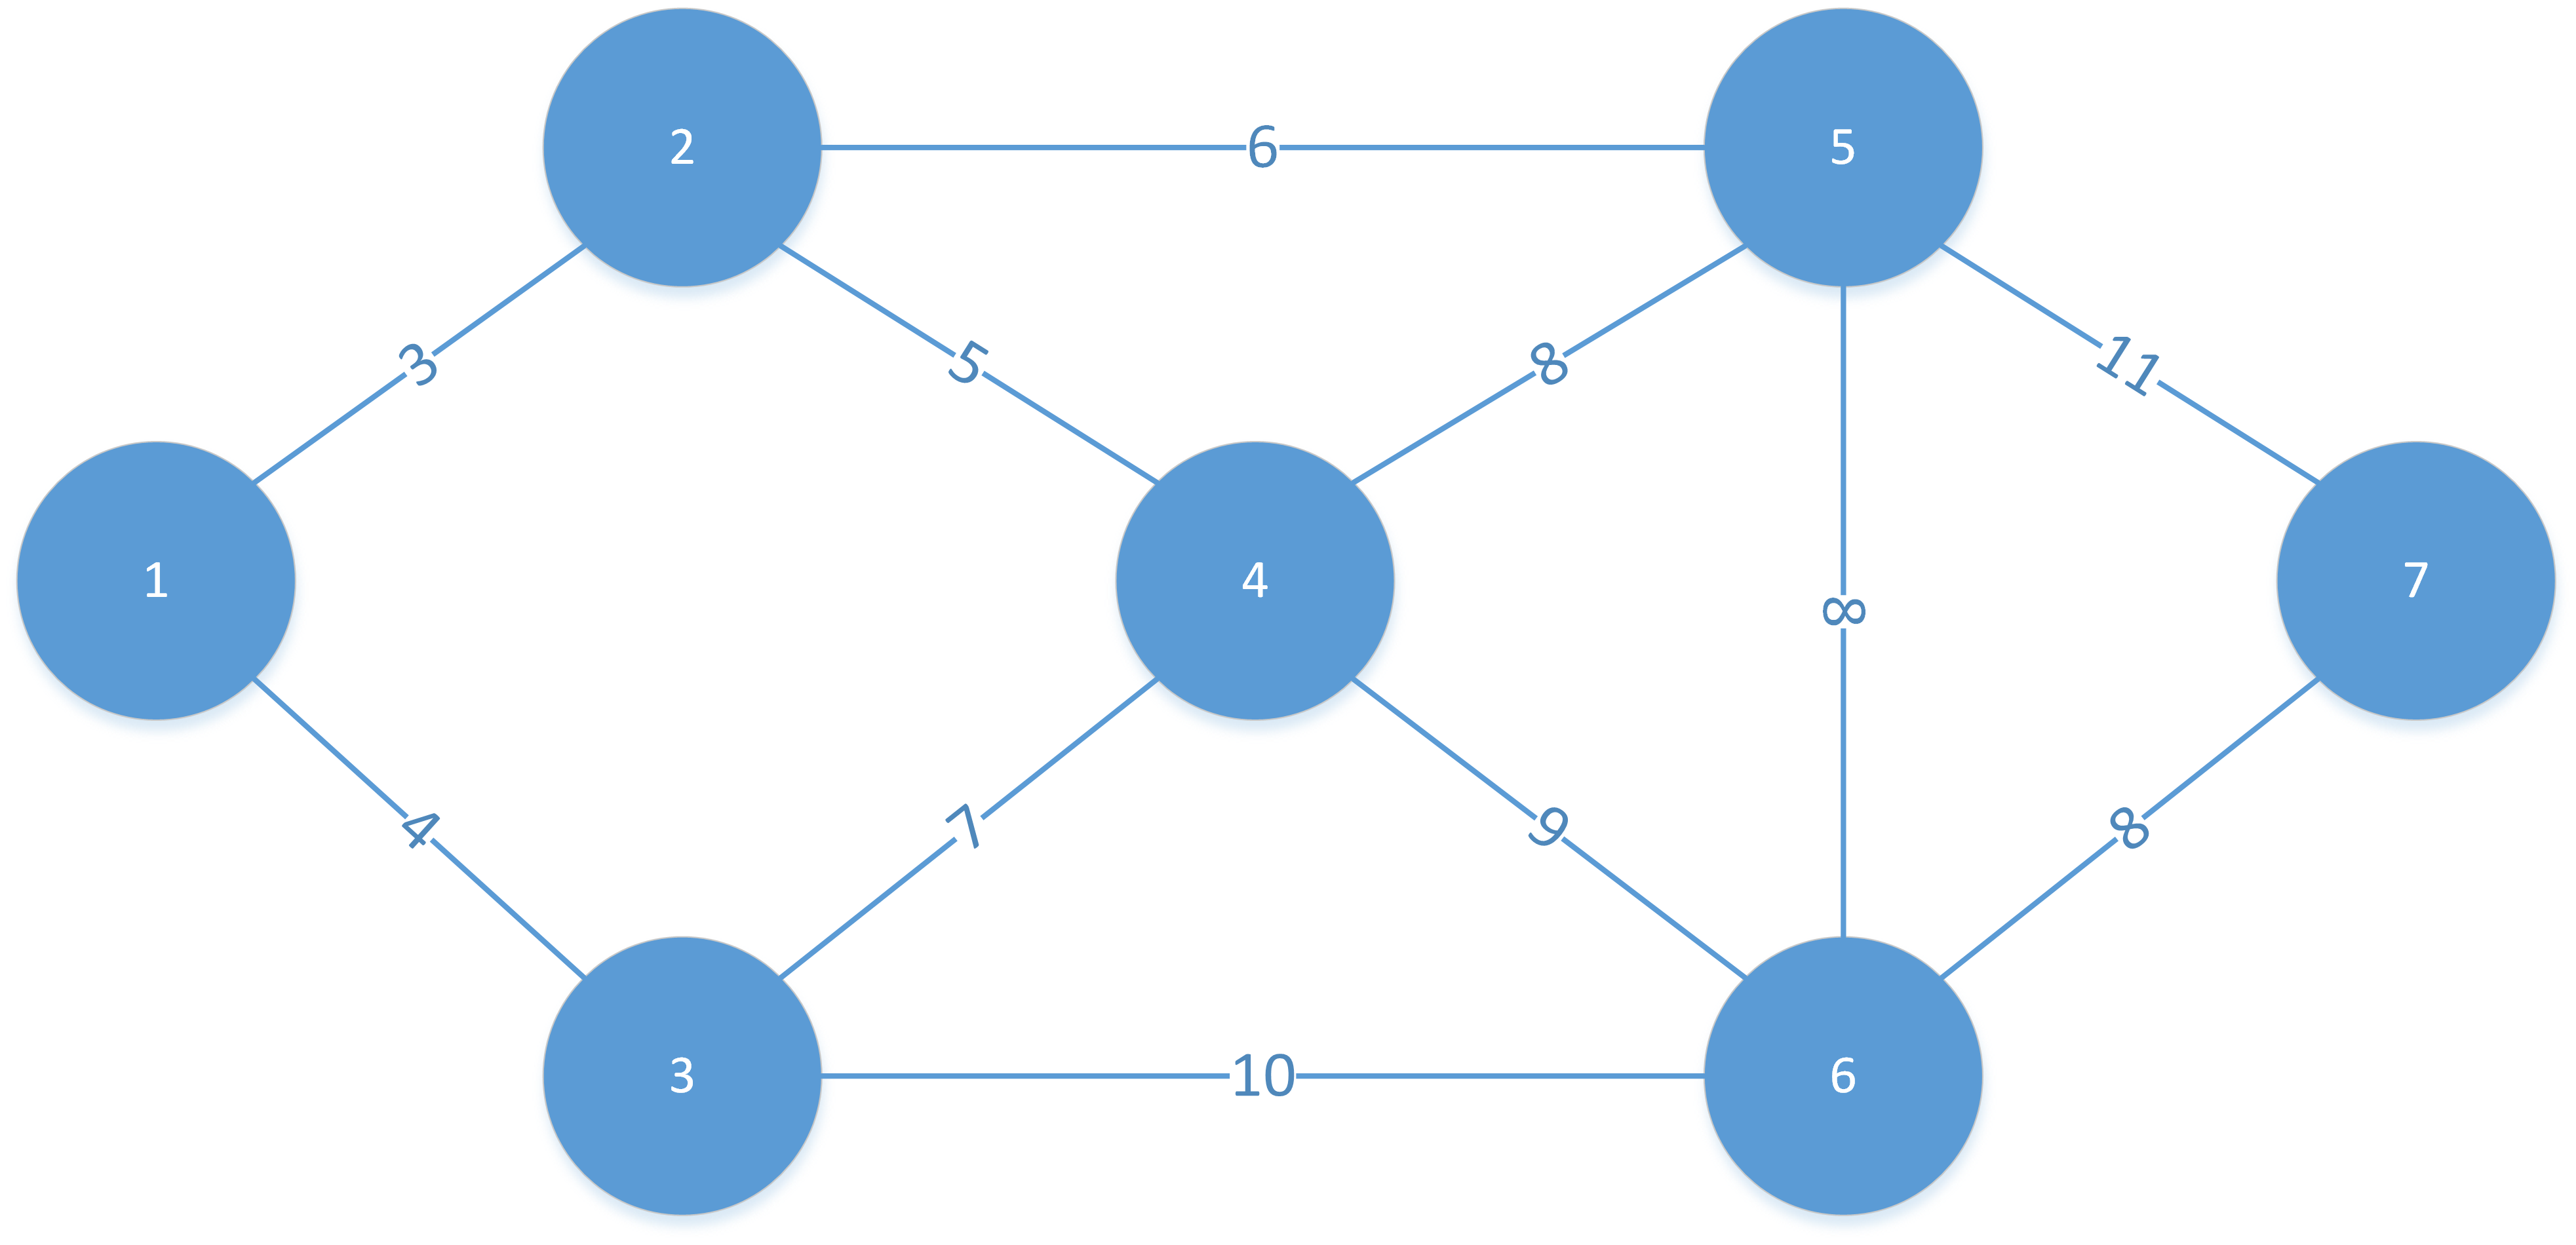
\includegraphics[scale=0.5]{dym.png}\\
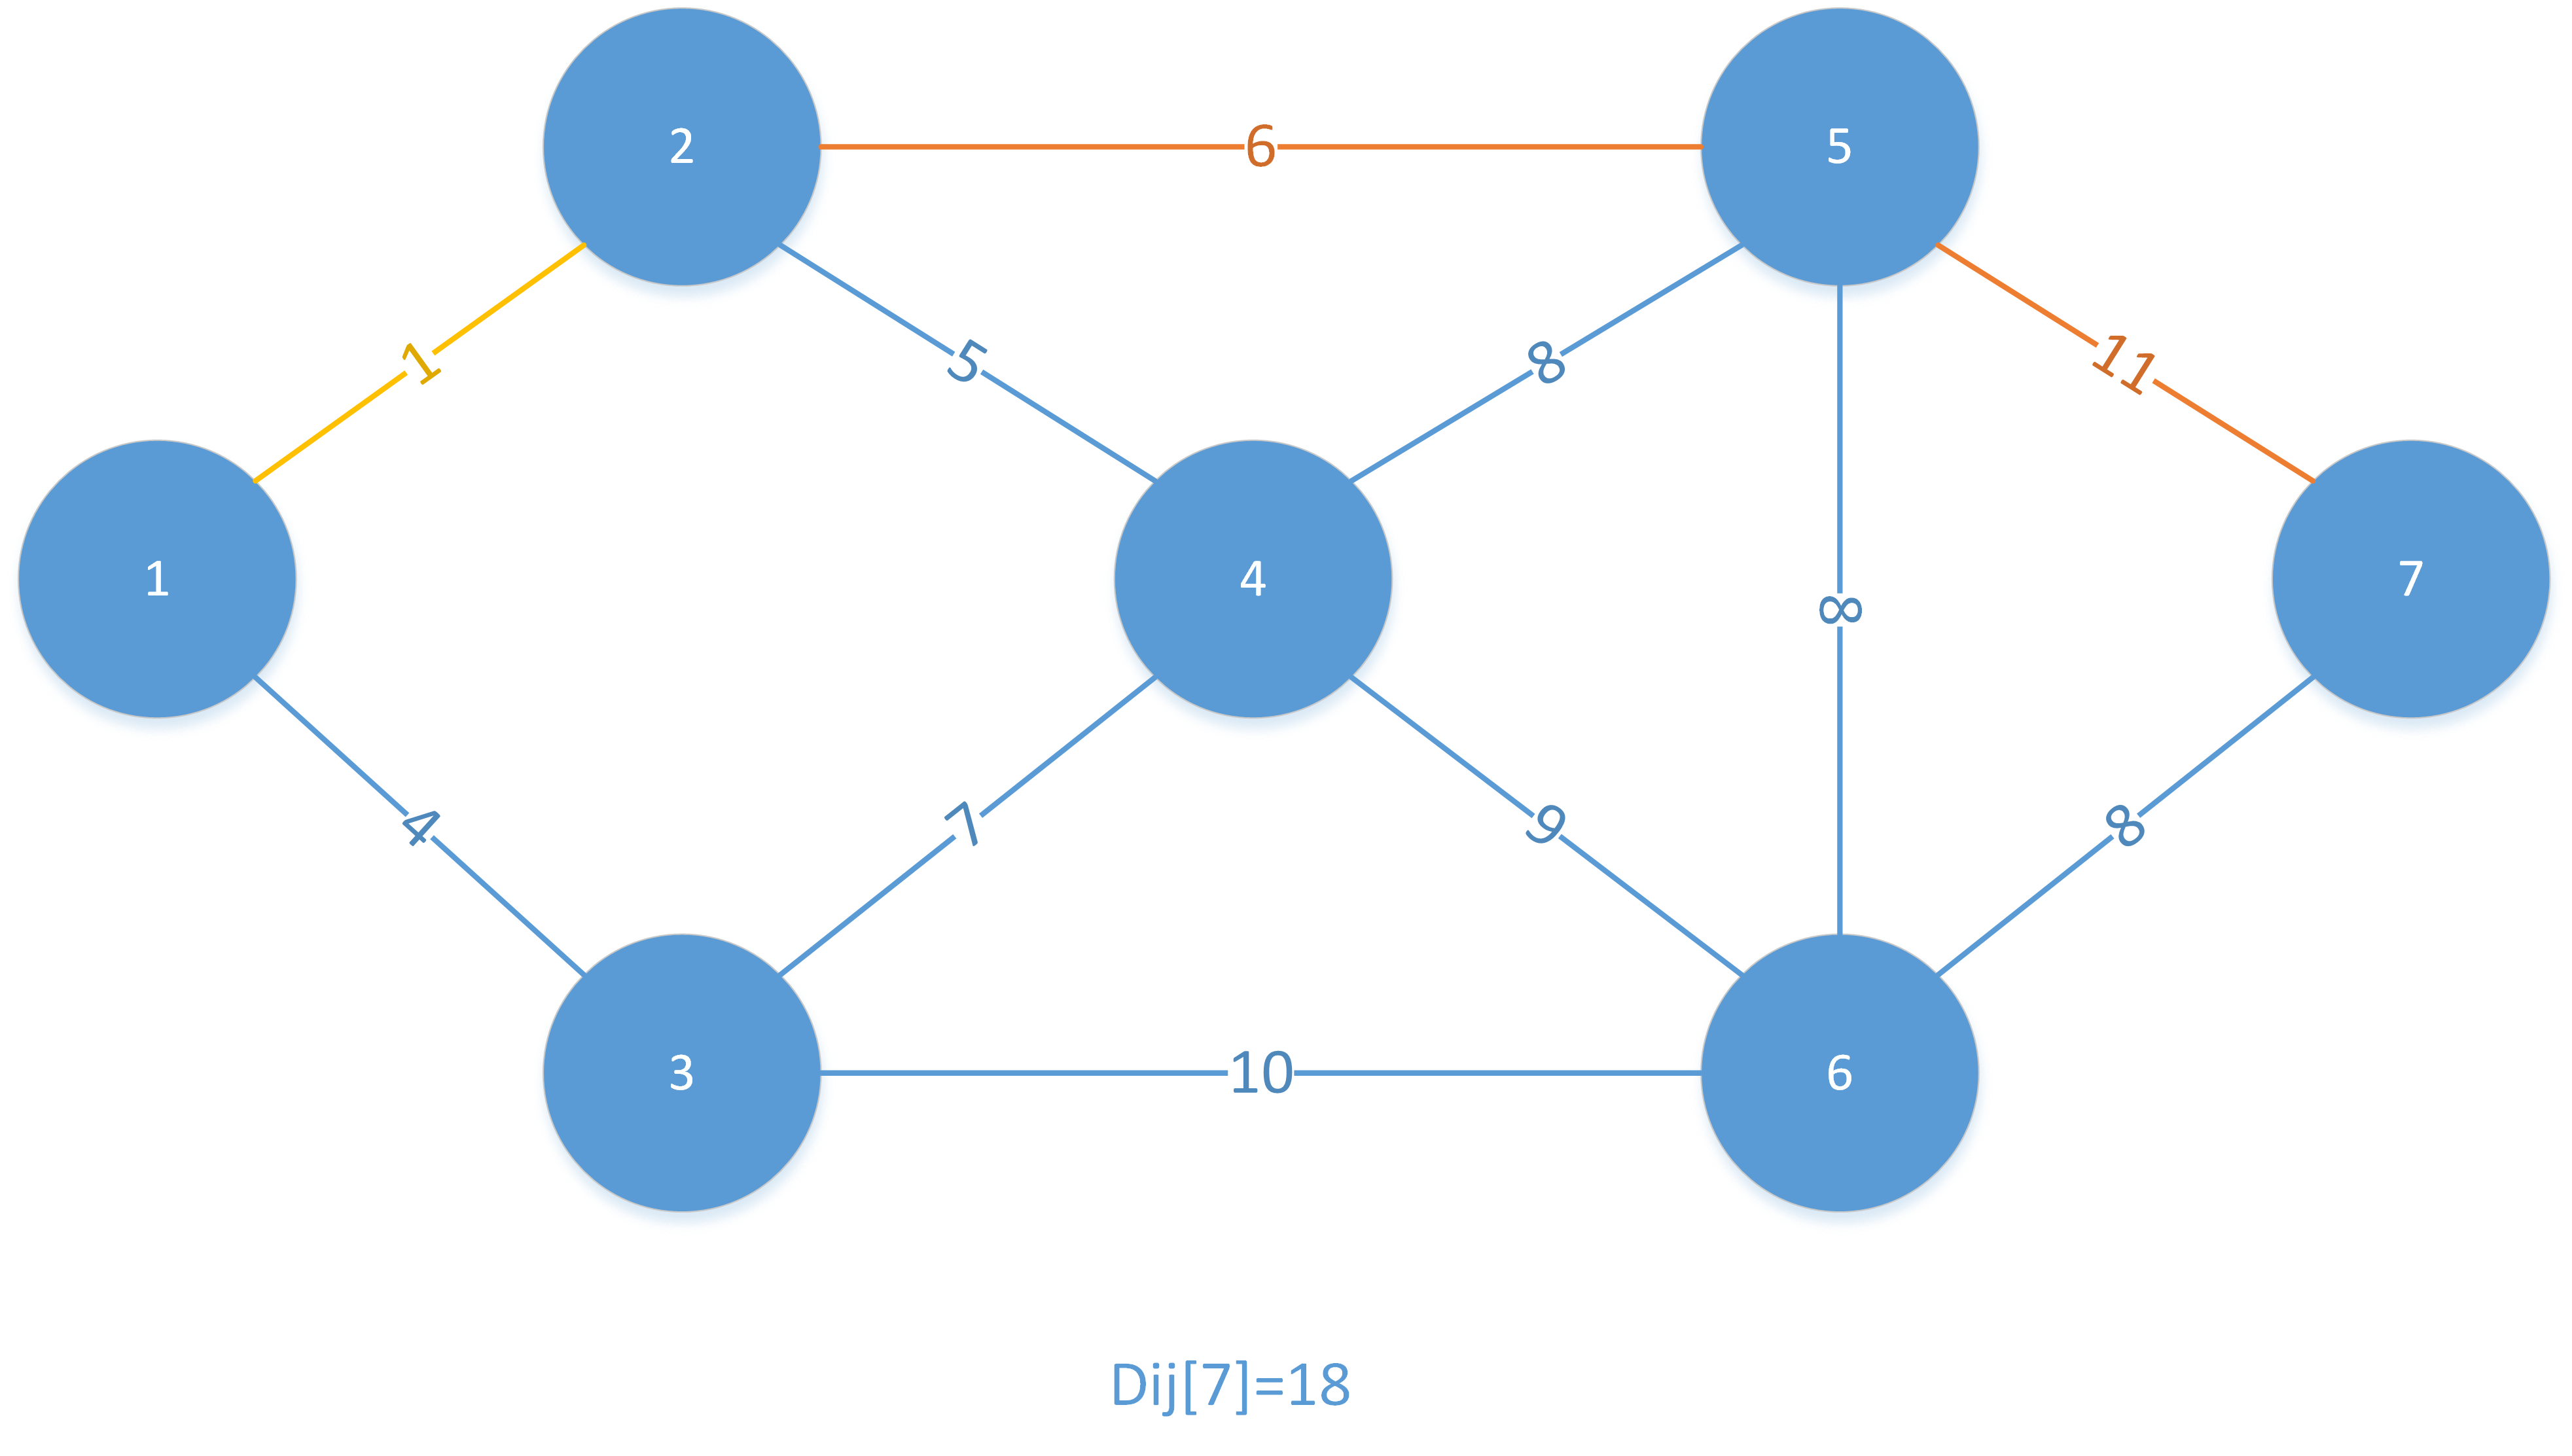
\includegraphics[scale=0.5]{dm3.png}\\
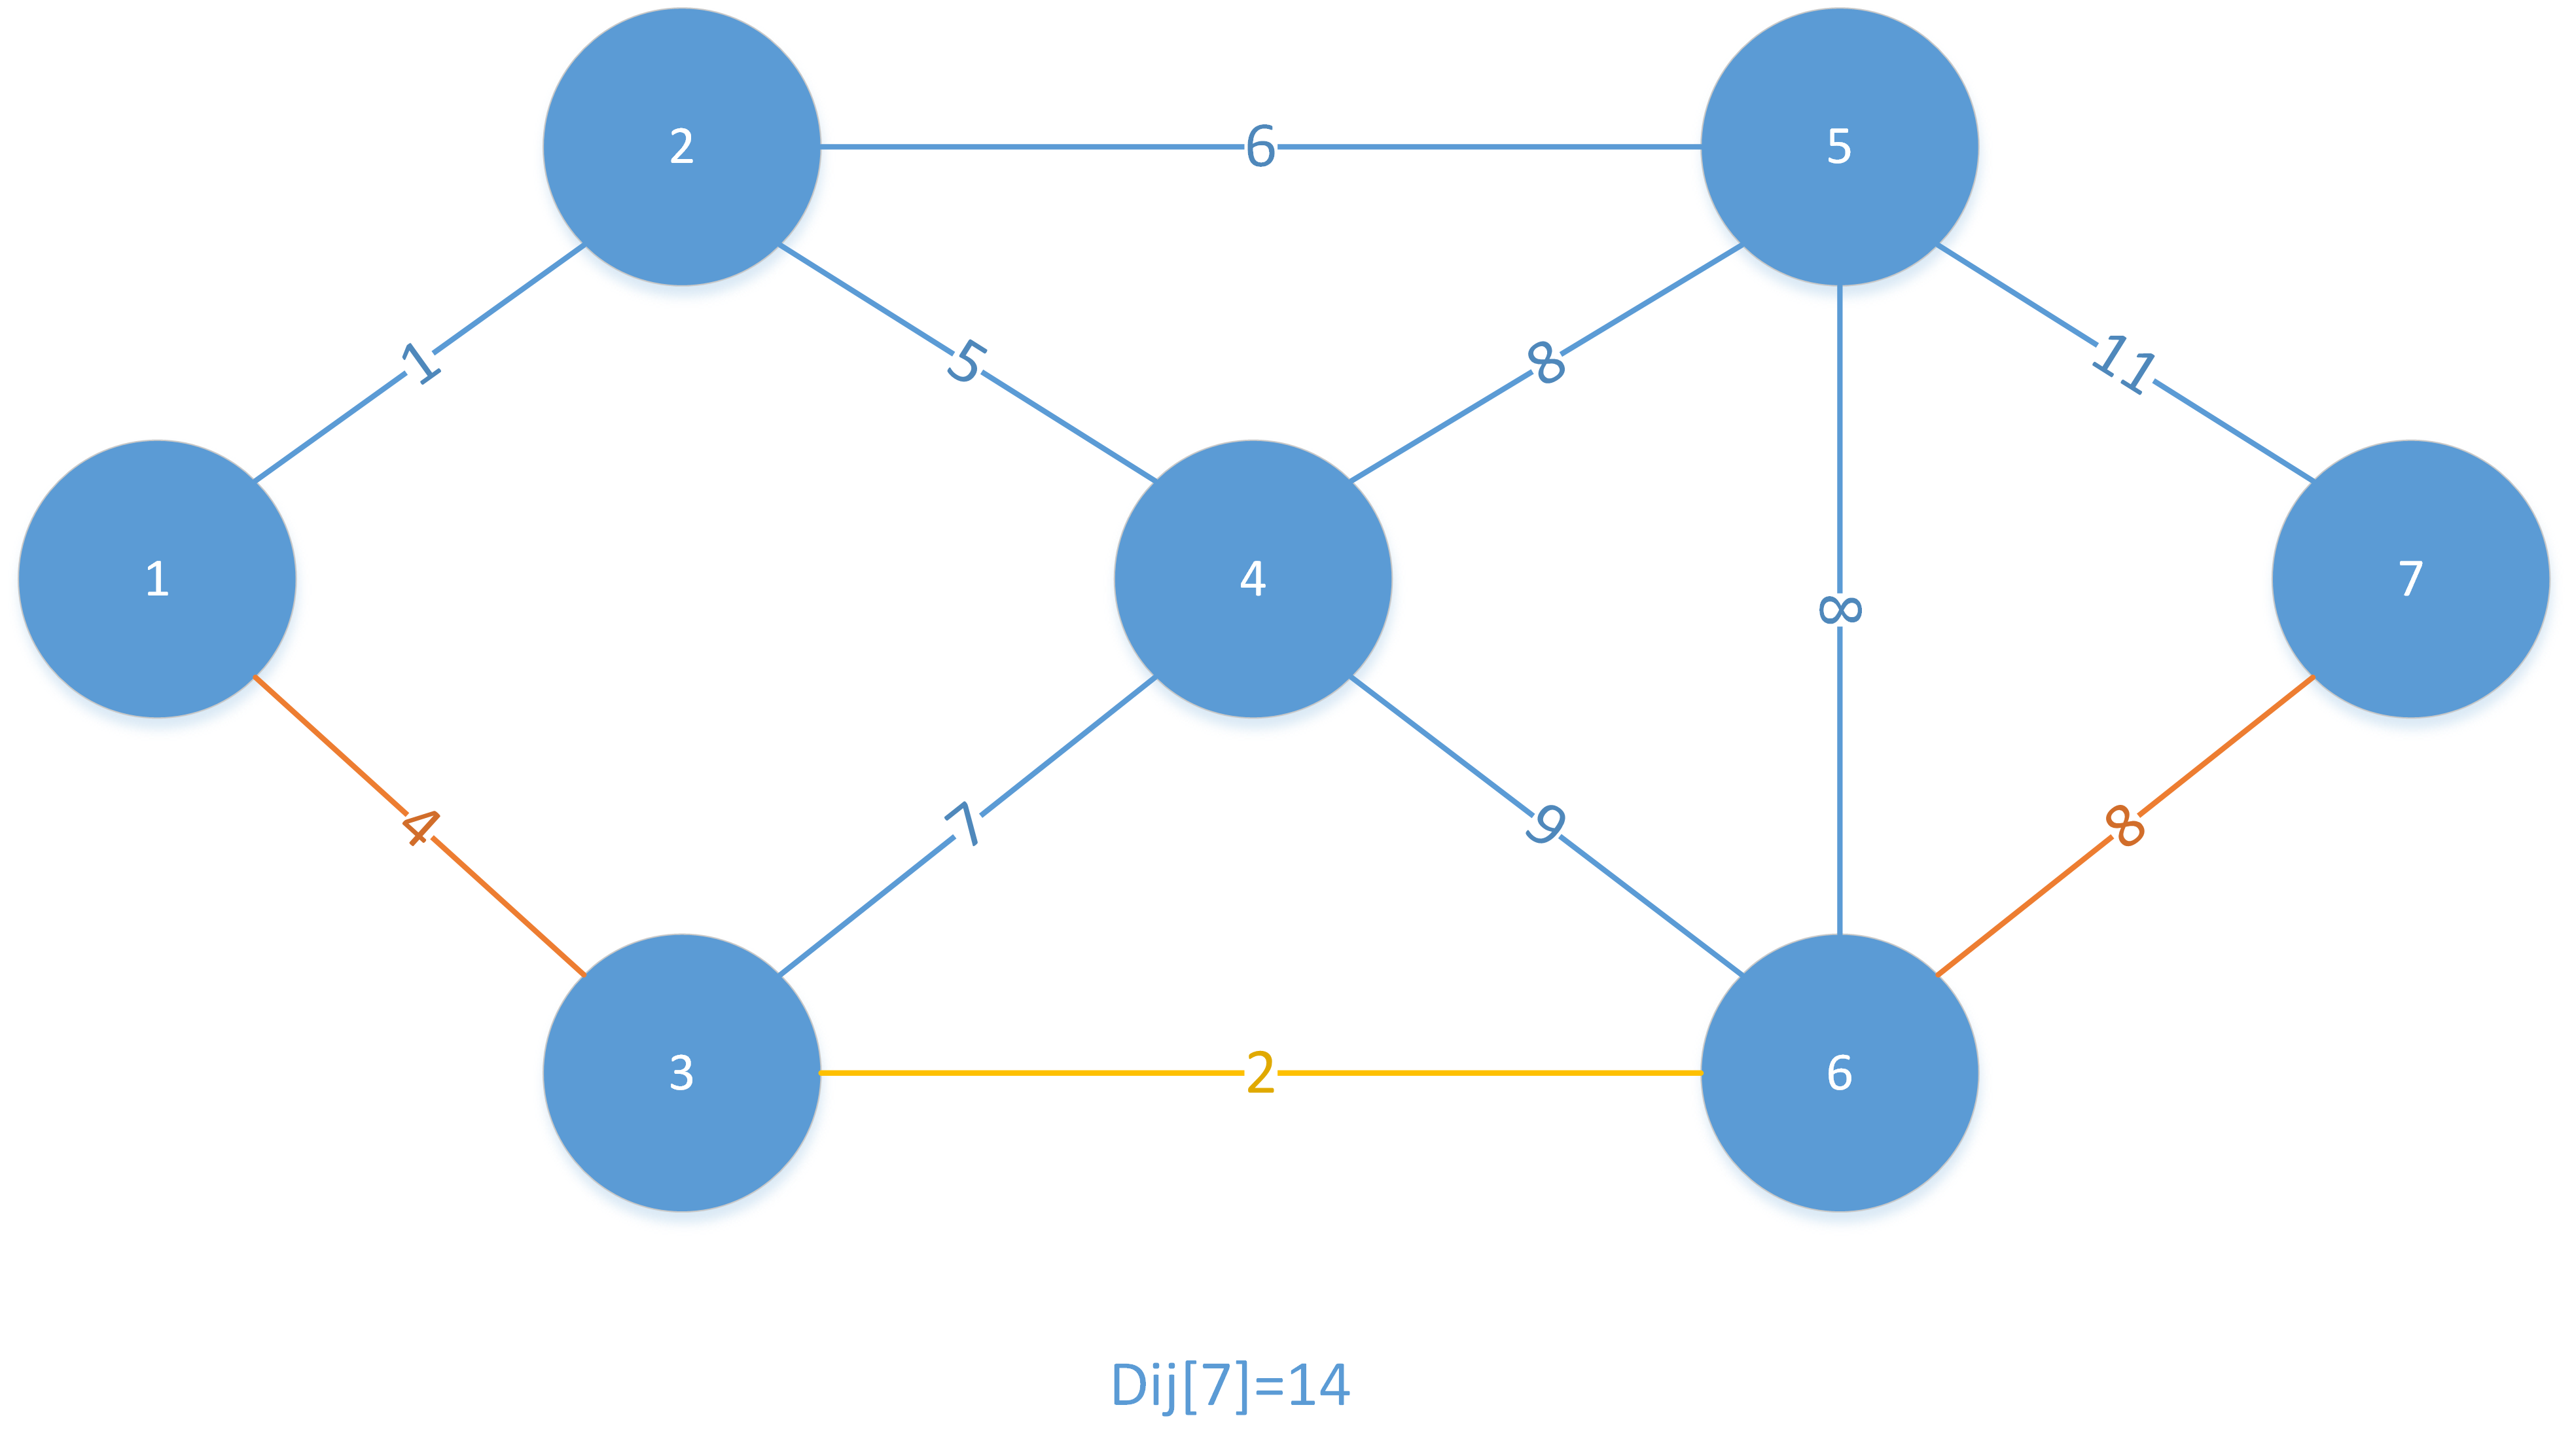
\includegraphics[scale=0.5]{dm4.png}
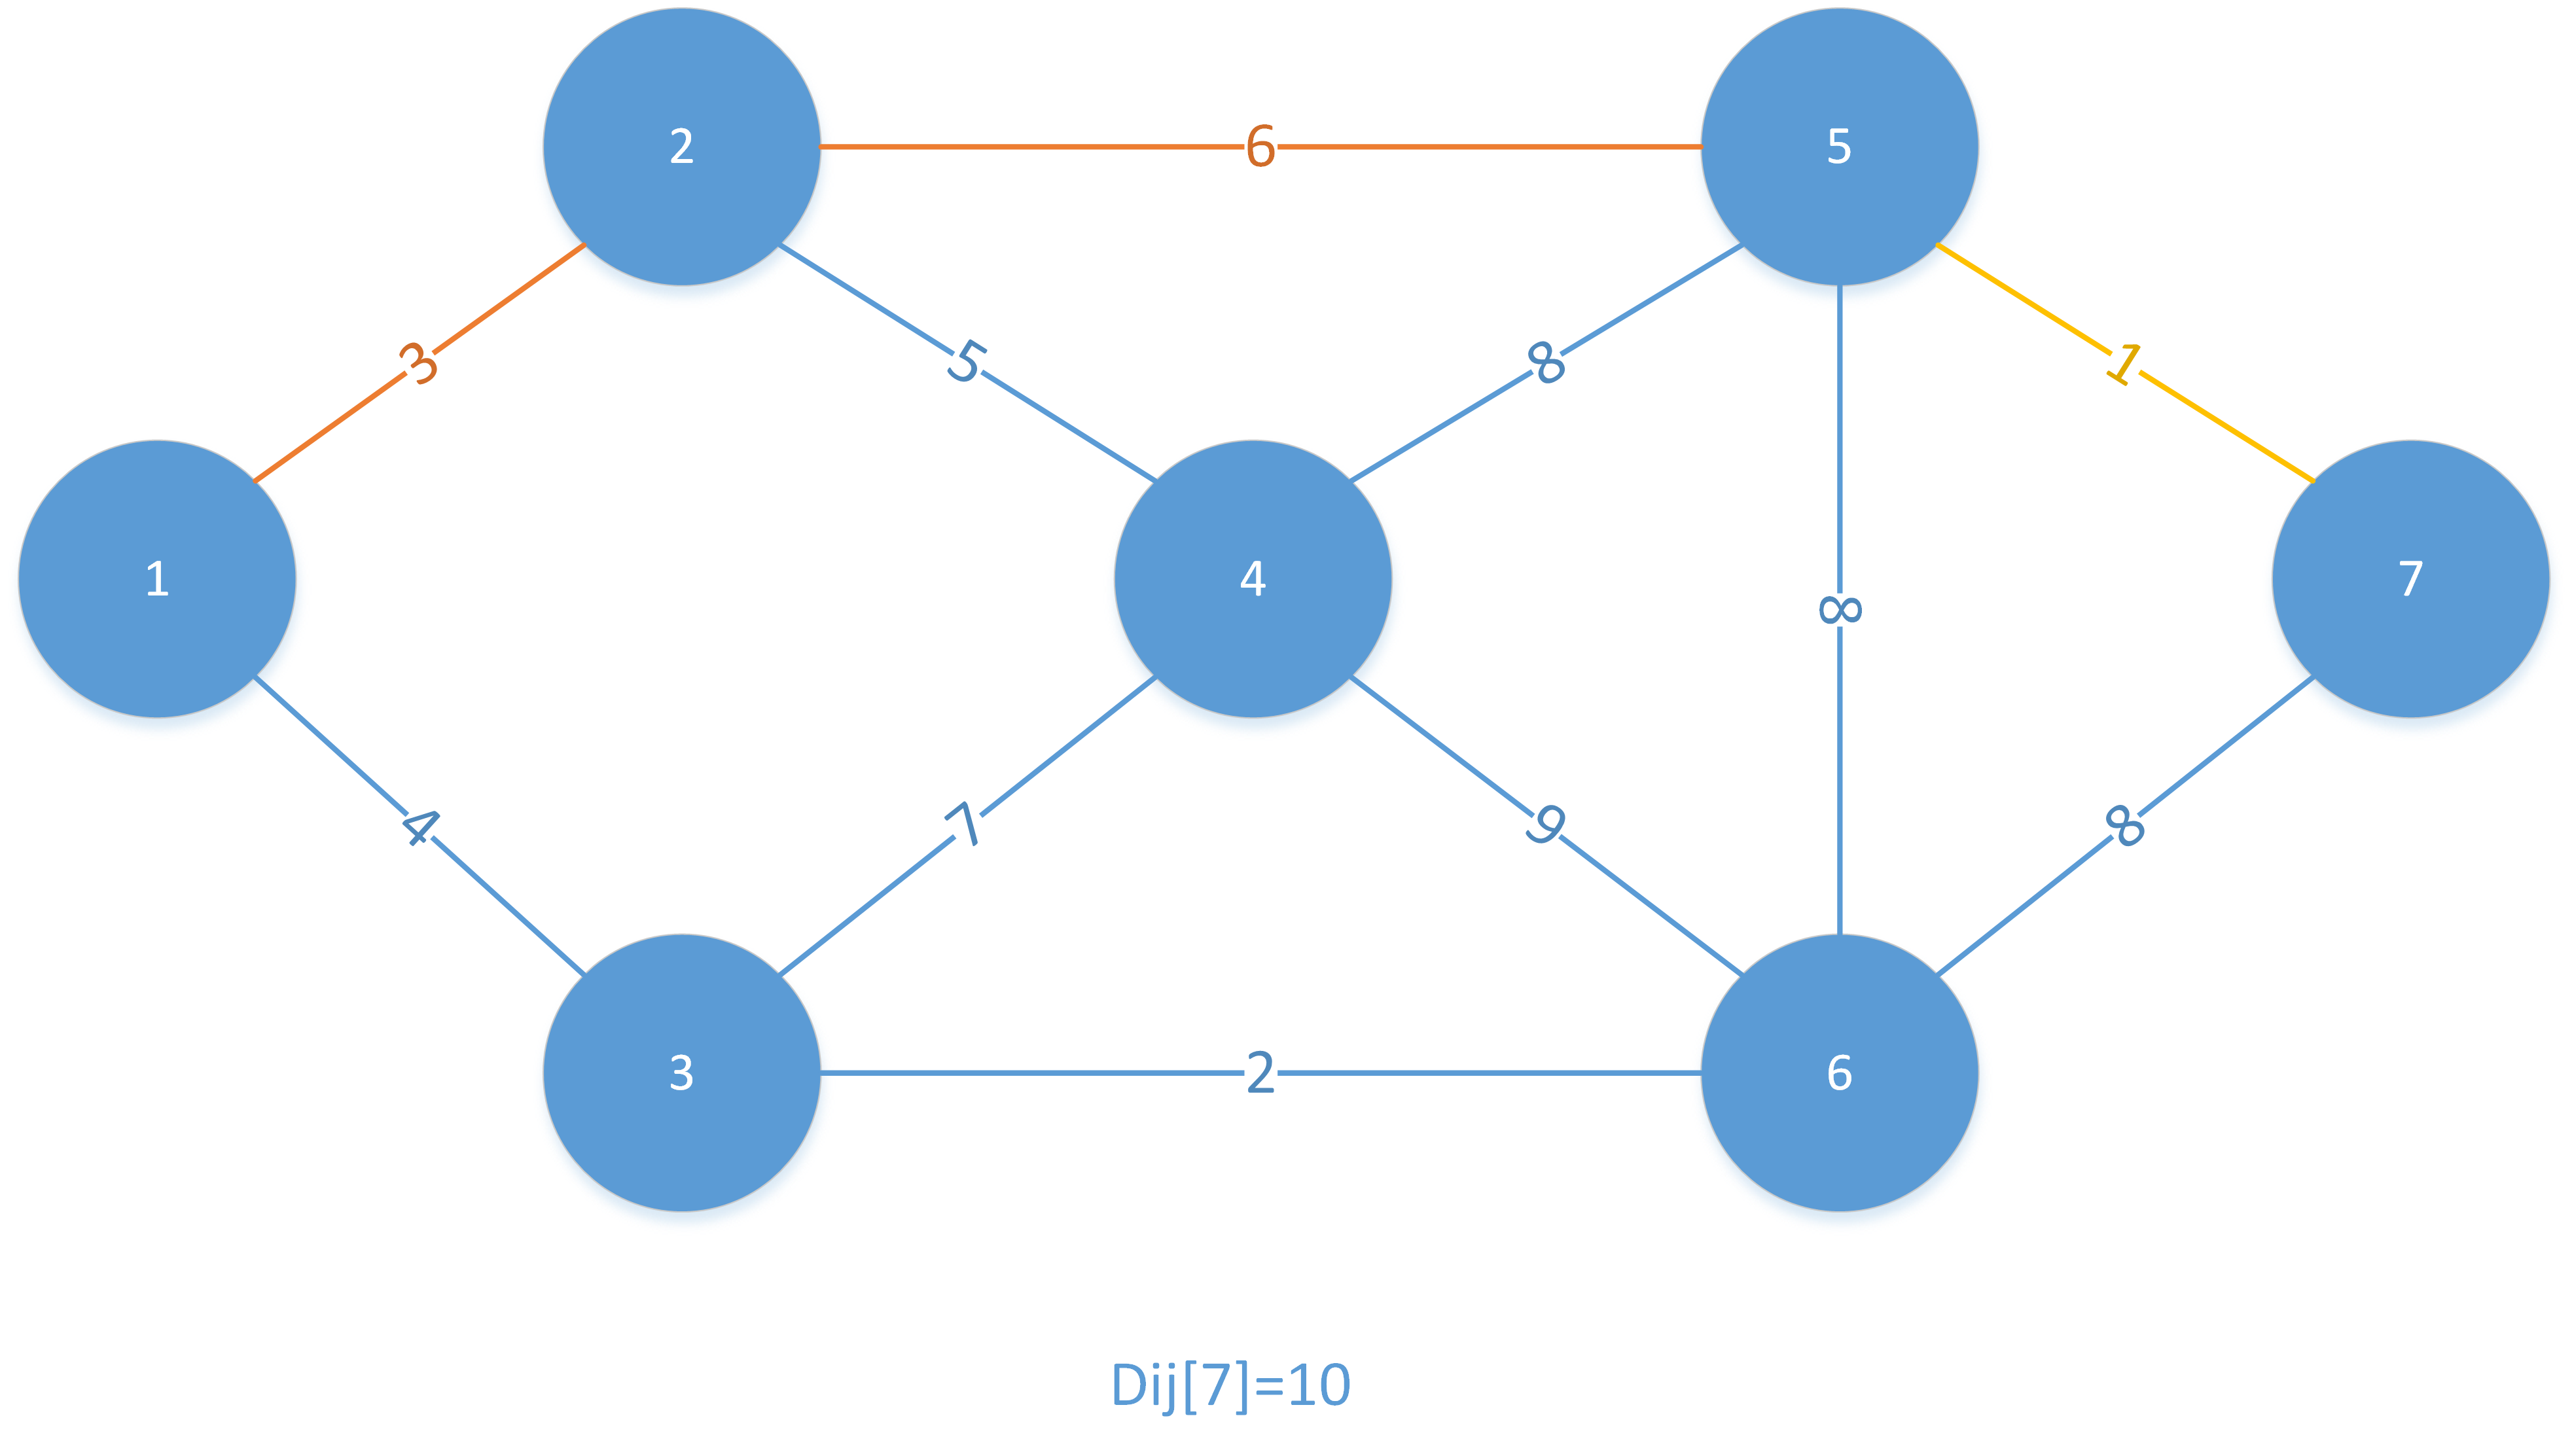
\includegraphics[scale=0.5]{dm5.png}\\
\textit{图四:结果图例说明}
\end{center}
\newpage
\section{Prim与Kruskral最小生成树算法选用}
\subsection{需求分析}
众所周知,有两种最小生成树的生成方法分别为Prim和Kruskral,由于不同的图的边稀疏程度不同,所以采用的两种时间复杂度有所差异,本实验将通过给定的图比较两种算法的优劣,并采用适用的算法,以减少时间浪费的问题。\\
\subsection{概述设计}
\textbf{\large{储备知识}}

首先,最小生成树是一副连通加权无向图中一棵权值最小的生成树。
主要可以使用Prim和Kruskal算法实现,对于稀疏图来说,用Kruskal写最小生成树效率更好,加上并查集,可对其进行优化。
Kruskal算法(并查集实现)\\
在使用Kruskal实现最小生成树之前,先来看下并查集需要注意的两点:
\begin{itemize}
\item 针对树可能会退化为链表的解决方案是,每次合并树时,总是将矮的树挂到高的树下,这种方式称为按秩合并。
\item 为了得到的树将更加扁平,加速以后直接或者间接引用节点的速度,Find时改变每一个节点的引用到根节点,这叫路径压缩。
\end{itemize}
Kruskal算法的步骤包括:
\begin{itemize}
    \item 对所有权值进行从小到大排序(这里对边排序时还需要记录边的索引,这样以边的权值排完序后只改变了权值的索引位置)
    \item 然后每次选取最小的权值,如果和已有点集构成环则跳过,否则加到该点集中。最终有所有的点集构成的树就是最佳的。
\end{itemize}
Prim算法(使用visited数组实现)
Prim算法求最小生成树的时候和边数无关,和顶点树有关,所以适合求解稠密网的最小生成树。

Prim算法的步骤包括:
\begin{itemize}
\item 将一个图分为两部分,一部分归为点集U,一部分归为点集V,U的初始集合为{V1},V的初始集合为{ALL-V1}。

\item 针对U开始找U中各节点的所有关联的边的权值最小的那个,然后将关联的节点Vi加入到U中,并且从V中删除(注意不能形成环)。

\item 递归执行步骤2,直到V中的集合为空。

\item U中所有节点构成的树就是最小生成树。
\end{itemize}
\textbf{\large{算法核心}}

方法上:Kruskal在所有边中不断寻找最小的边,Prim在U和V两个集合之间寻找权值最小的连接,共同点是构造过程都不能形成环。

时间上:Prim适合稠密图,复杂度为O(n * n),因此通常使用邻接矩阵储存,复杂度为O(e * loge),而Kruskal多用邻接表,稠密图 Prim > Kruskal,稀疏图 Kruskal > Prim。

空间上: Prim适合点少边多,Kruskal适合边多点少。
\subsection{设计实现}
\begin{lstlisting}
    #include<bits/stdc++.h>
    using namespace std;
    const int maxn=50;
    const int INF=0x3f3f3f3f;
    struct node{int from,to,cost;}edge[maxn];
    int par[maxn];
    int gr[maxn][maxn];
    bool visp[maxn];
    bool acte[maxn][maxn];
    bool vise[maxn][maxn];
    int st,tot,n,m;
    int find(int num)
    {
        return par[num]==num?num:par[num]=find(par[num]);
    }
    int cmp(const void *a,const void *b)
    {
        return(((node*)a)->cost-((node*)b)->cost);
    }
    
    void init()
    {
        int a,b,c;
        memset(visp,sizeof(visp),false);
        memset(acte,sizeof(acte),false);
        memset(vise,sizeof(vise),false);
        cin>>n>>m;
        for (int i=0;i<maxn;i++)
         for (int j=0;j<maxn;j++)
            gr[i][j]=INF;
        cout<<"please input the (v,w) and value:"<<endl;
        for (int i=1;i<=m;i++)
        {
            cin>>a>>b>>c;
            gr[a][b]=c;
            gr[b][a]=c;
        }
        cout<<"please input the start point:"<<endl;
        cin>>st;
        visp[st]=true;
        for (int i=1;i<=n;i++)
            if (visp[i]==false&&gr[st][i]!=INF)  acte[st][i]=true;
        tot=1;
    }
    void merge()
    {
        while (tot<n)
        {
            int l=INF,p,v,w;
            for (int i=1;i<=n;i++)
                for (int j=1;j<=n;j++)
                if (gr[i][j]!=INF&& acte[i][j] && !(visp[i]&&visp[j]))
                 if (l>gr[i][j]) 
                    { if (visp[i]&&!visp[j]) {p=j;l=gr[i][j];v=i;w=j;} if (!visp[i]&&visp[j]) {p=i;l=gr[i][j];v=i;w=j;}}
            visp[p]=true;
            cout<<p;
            vise[v][w]=true;
            tot++;
            for (int i=1;i<=n;i++)
                if (visp[i]==false&&gr[p][i]!=INF) acte[p][i]=true;
        }
    }
    void prim()
    {
        init();
        int ans=0;
        merge();
        for (int i=1;i<=n;i++)
            for (int j=1;j<=n;j++)
            if (vise[i][j]) 
                {
                    cout<<i<<'-'<<j<<endl;
                    ans+=gr[i][j];
                }
        cout<<"total value:"<<ans;
    }
    int main()
    {
        cin>>n>>m;
        if (n*n>m*log(m))
        {
            cout<<"Use kruskal algorithm"<<endl;
            for(int i=0;i<=n;i++)
                par[i]=i;
            for(int i=0;i<m;i++)
                scanf("%d%d%d",&edge[i].from,&edge[i].to,&edge[i].cost);
            qsort(edge,m,sizeof(node),cmp);
            int cnt=0,res=0;
            for(int i=0;i<m;i++)
            {
                int sa=find(edge[i].from),sb=find(edge[i].to);
                if(sa==sb)
                    continue;
                res+=edge[i].cost;
                par[sa]=sb;
                cnt++;
                if(cnt==n-1)
                    break;
            }
            if(cnt>=n-1)
                printf("%d\n",res);
            else
                printf("?\n");
        }
        else {
            cout<<"Use prim algorithm"<<endl;
            prim();
        }
        return 0;
    }
    /*
    input:
    6 9
    1 2 6
    1 3 3
    2 3 2
    2 4 5
    3 4 3
    4 6 3
    4 5 2
    3 5 4
    5 6 5
    */
\end{lstlisting}
\subsection{设计调试和测试结果说明}
输入:\\
首先第一行是两个正整数代表图的点数和边数,之后输入每条边的关联点和权值\\

输出:\\ 
返回使用的方法名称(Prim or Kruskal)\\
\begin{center}
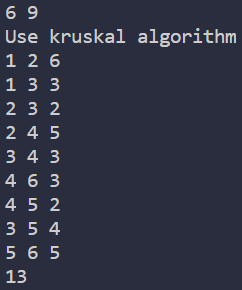
\includegraphics[scale=0.6]{prim_kruskral.png}\\
\textit{图五:测试结果}\\
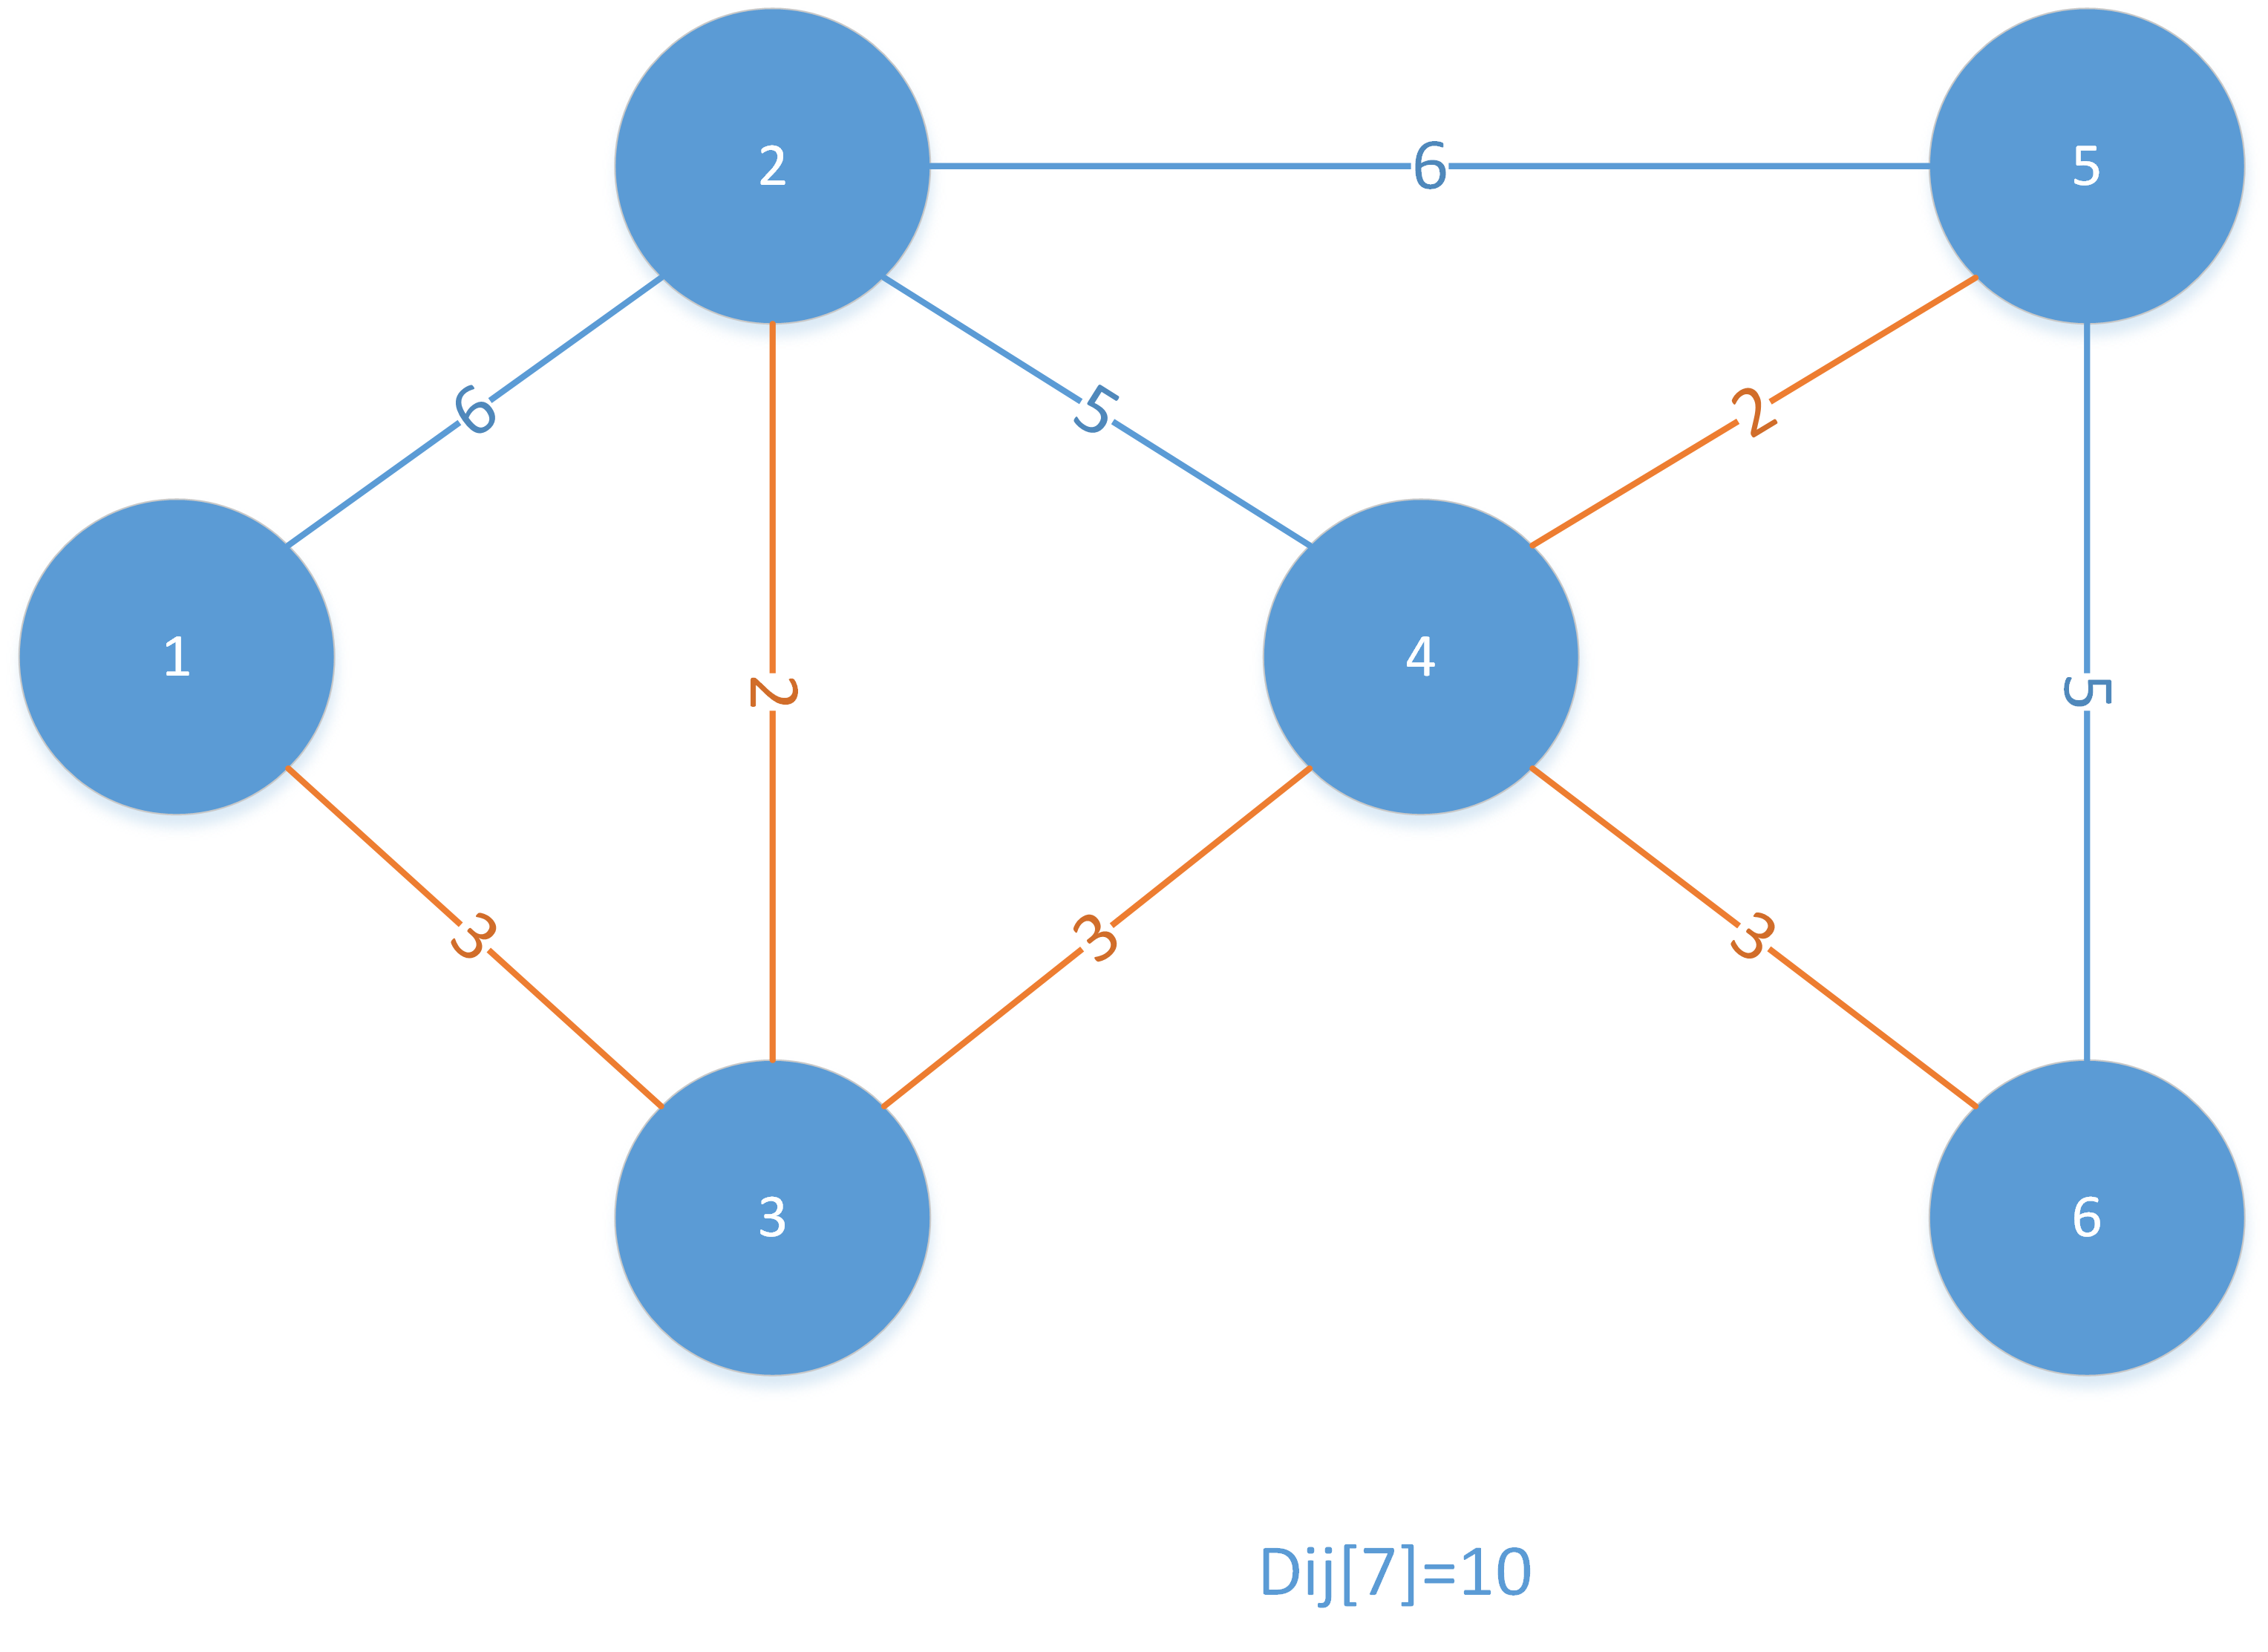
\includegraphics[scale=0.6]{tree.png}\\
\textit{图六:测试结果说明}\\
\end{center}
\newpage
\section{二维高斯函数插值}
\subsection{需求分析}
已知二维高斯函数:
$$
f(x,y)=\frac{1}{2\pi \sigma_1\sigma_2\sqrt{1-\rho^2}}e^{-\frac{1}{2(1-\rho^2)}(\frac{(x-\mu_1)^2}{\sigma_1^2}-\frac{2\rho(x-\mu_1)(y-\mu_2)}{\sigma_1\sigma_2}+\frac{(y-\mu_2)^2}{\sigma_2^2})}
$$
能否根据一组边界值,直接无误差地得到边界内部所有离散点的值呢?
\subsection{概述设计}
由Coons曲面生成原理,记矩形$\Omega$的四个顶点$P_1(x_0,y_0)$,$P_2(x_1,y_0)$,$P_3(x_1,y_1)$,$P_R(x_0,y_1)$。设Q(x,y)是$\Omega$内任意一个计算点,经过Q作矩形平行的平行线,平行线和边界交点分别是
$Q_1(x,y_0)$,$Q_2(x_1)$,$Q_3(x,y_1)$,$Q_4(x_0,y)$,如果F(x,y)在 边界上连续,则Coons插值是:
$F(Q)=\sum_{i=1}^{4} \frac{A_i+A_{i+1}}{A}f(Q_i)-\sum_{i=1}^{4} \frac{A_i}{A} f(P_i)$
其中$A_1=A_5=(x_1-x)(y_1-y)$,
$A_2=(x-x_0)(y_1-y)$,
$A_3=(x-x_0)(y-y_0)$,
$A_4=(x_1-x)(y-y_0)$,
$A_5=A_1$,
$A=(x_1-x_0)(y_1-y_0)$,
从而$A=A_1+A_2+A_3+A_4$\\
\begin{center}
    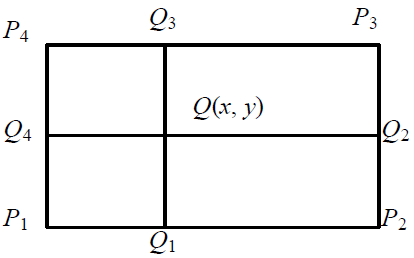
\includegraphics[scale=0.6]{conns.png}\\
    \textit{图六:Conns曲面生成区域}
\end{center}
由于已知边界条件,得到的中心点的坐标对应的f(x,y),可以通过去密集的离散点,得到整个边界内的分布。
\subsection{设计实现}
\begin{lstlisting}
    from mpl_toolkits import mplot3d
import matplotlib.pyplot as plt
import matplotlib 
import numpy as np
import math 
sigma1=float(input('σ1:'))
mu1=float(input('μ1:'))
sigma2=float(input('σ2:'))
mu2=float(input('μ2:'))
rho=float(input('ρ:'))
x0=float(input('x0:'))
y0=float(input('y0:'))
x1=float(input('x1:'))
y1=float(input('y1:'))
def r(x, y):
    return np.sqrt(x**2+y**2)
def p(xi,yi):
    return np.log(1/(2*math.pi*sigma1*sigma2*math.sqrt(1-rho**2))*np.exp(-1/(2*math.sqrt(1-rho**2))*(((xi-mu1)/sigma1)**2+((yi-mu2)\
    /sigma2)**2-2*rho*(xi-mu1)*(yi-mu2)/(sigma1*sigma2))))
def f(x,y):
    g=0
    A=(x1-x0)*(y1-y0)
    Ai=[]
    fq=[]
    fp=[]
    Ai=Ai+[(x1-x)*(y1-y)]+[(x-x0)*(y1-y)]+[(x-x0)*(y-y0)]+[(x1-x)*(y-y0)]
    fq=fq+[p(x,y0)]+[p(x1,y)]+[p(x,y1)]+[p(x0,y)]
    fp=fp+[p(x0,y0)]+[p(x1,y0)]+[p(x1,y1)]+[p(x0,y1)]
    for i in range(4):
        g=g+(Ai[i]+Ai[(i+1)%4])*fq[i]-Ai[i]*fp[i]        
    return np.exp(g/A)
x = np.linspace(x0+0.01,x1-0.01,100)
y = np.linspace(x0+0.01,y1-0.01,100)
X, Y = np.meshgrid(x, y)
Z = f(X,Y)
plt.figure(1)
ax = plt.axes(projection='3d')
ax.plot_surface(X, Y, Z, rstride=1, cstride=1, cmap='viridis', edgecolor='none')
ax.set_title('interp2 f(x,y)')
ax.set_xlabel('x')
ax.set_ylabel('y')
ax.set_zlabel('z')
x = np.linspace(x0+0.01,x1-0.01,100)
y = np.linspace(x0+0.01,y1-0.01,100)
X, Y = np.meshgrid(x, y)
Z = np.exp(p(X,Y))
plt.figure(2)
ax = plt.axes(projection='3d')
ax.plot_surface(X, Y, Z, rstride=1, cstride=1, cmap='viridis', edgecolor='none')
ax.set_title('function f(x,y)')
ax.set_xlabel('x')
ax.set_ylabel('y')
ax.set_zlabel('z')
plt.show()
\end{lstlisting}
\subsection{测试结果与说明}
\begin{center}
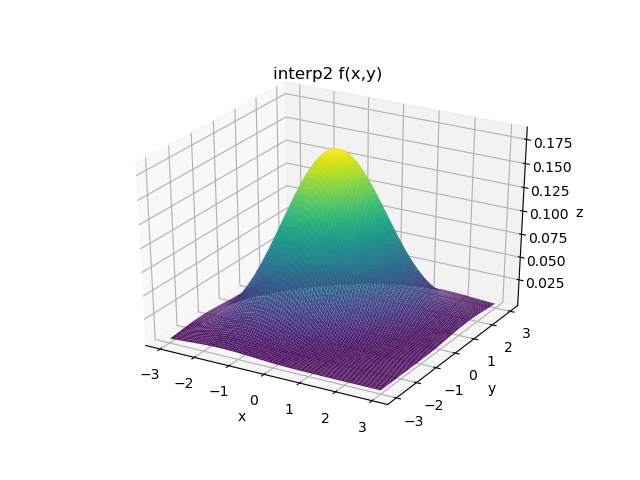
\includegraphics[scale=0.5]{Figure_1.png}
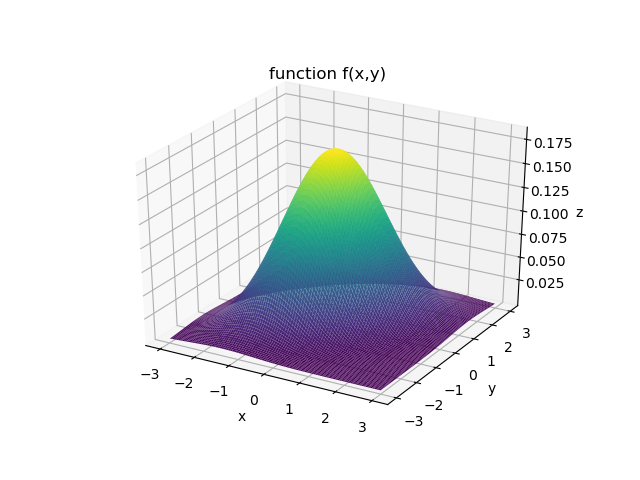
\includegraphics[scale=0.5]{Figure_2.png}\\
\textit{图七:插值绘图和函数绘图的比较}
根据绘出的[-3 3 -3 3]之间的图可以看出,插值和函数的绘图较为吻合,在一定程度上反映了理论的正确性。\\
\end{center}
\textit{参考文献:二元正态分布函数(Coons 曲面法)插值研究  邱 钧 孙洪泉 韩 伟 工程图学学报 2002.Nov.3 2-6}
\newpage
\section{找对象算法}
\subsection{需求分析}
在一定的匹配问题下,如何才能使尽量多的对象能够进行匹配,并且达到最优呢?
极大匹配(Maximal Matching)是指在当前已完成的匹配下,无法再通过增加未完成匹配的边的方式来增加匹配的边数。最大匹配(maximum matching)是所有极大匹配当中边数最大的一个匹配。选择这样的边数最大的子集称为图的最大匹配问题。
如果一个匹配中,图中的每个顶点都和图中某条边相关联,则称此匹配为完全匹配,也称作完备匹配。
求二分图最大匹配可以用最大流(Maximal Flow)或者匈牙利算法(Hungarian Algorithm)
\subsection{概述设计}
设M是图G=(V,E)的一个匹配,vi∈V。若vi与M中的边相关联,则称vi是M饱和点,否则称vi为M非饱和点。 如果G中每个顶点都是M饱和点,则称M为G的完美匹配。 设M是G的一个匹配,P是G的一条链。如果P的边交替地一条是M中的边,一条不是M中的边,则称P为M交错链。类似地,我们可以定义G的交错圈。易知,G的交错圈一定是偶圈。 一条连接两个不同的M非饱和点的M交错链称为M增广链。 两个集合S1与S2的“异或”操作S1⊕S2是指集合S1⊕S2=(S1∩S2)-(S1∪S2) 容易看出,设M是G的匹配,P是G中的M增广链、则M⊕P也是G的匹配,而且 可以证明,G中匹配M是最大匹配当且仅当G中没有M增广链。
如果一个图是连通的,可以用如下的方法判定是否是二分图:
在图中任选一顶点v,定义其距离标号为0,然后把它的邻接点的距离标号均设为1,接着把所有标号为1的邻接点均标号为2(如果该点未标号的话),如图所示,以此类推。
标号过程可以用一次BFS实现。标号后,所有标号为奇数的点归为X部,标号为偶数的点归为Y部。
接下来,二分图的判定就是依次检查每条边,看两个端点是否是一个在X部,一个在Y部。
如果一个图不连通,则在每个连通块中作判定。\\

选择边数最大的子图称为图的最大匹配问题(maximal matching problem)
如果一个匹配中,图中的每个顶点都和图中某条边相关联,则称此匹配为完全匹配,也称作完备匹配。
图中所示为一个最大匹配,但不是完全匹配。
由增广路的定义可以推出下述三个结论:
\begin{itemize}
    \item P的路径长度必定为奇数,第一条边和最后一条边都不属于M,因为两个端点分属两个集合,且未匹配。
    \item P经过取反操作可以得到一个更大的匹配M’。
    \item M为G的最大匹配当且仅当不存在相对于M的增广路径。
\end{itemize}
\subsection{设计实现}
\begin{lstlisting}
    import itertools
import numpy as np
from numpy import random
from scipy.optimize import linear_sum_assignment

class TaskAssignment:
 
    # 类初始化,需要输入参数有任务矩阵以及分配方式,其中分配方式有两种,全排列方法all_permutation或匈牙利方法Hungary。
    def __init__(self, task_matrix, mode):
        self.task_matrix = task_matrix
        self.mode = mode
        if mode == 'all_permutation':
            self.min_cost, self.best_solution = self.all_permutation(task_matrix)
        if mode == 'Hungary':
            self.min_cost, self.best_solution = self.Hungary(task_matrix)
 
    # 全排列方法
    def all_permutation(self, task_matrix):
        number_of_choice = len(task_matrix)
        solutions = []
        values = []
        for each_solution in itertools.permutations(range(number_of_choice)):
            each_solution = list(each_solution)
            solution = []
            value = 0
            for i in range(len(task_matrix)):
                value += task_matrix[i][each_solution[i]]
                solution.append(task_matrix[i][each_solution[i]])
            values.append(value)
            solutions.append(solution)
        min_cost = np.min(values)
        best_solution = solutions[values.index(min_cost)]
        return min_cost, best_solution
 
    # 匈牙利方法
    def Hungary(self, task_matrix):
        b = task_matrix.copy()
        # 行和列减0
        for i in range(len(b)):
            row_min = np.min(b[i])
            for j in range(len(b[i])):
                b[i][j] -= row_min
        for i in range(len(b[0])):
            col_min = np.min(b[:, i])
            for j in range(len(b)):
                b[j][i] -= col_min
        line_count = 0
        # 线数目小于矩阵长度时,进行循环
        while (line_count < len(b)):
            line_count = 0
            row_zero_count = []
            col_zero_count = []
            for i in range(len(b)):
                row_zero_count.append(np.sum(b[i] == 0))
            for i in range(len(b[0])):
                col_zero_count.append((np.sum(b[:, i] == 0)))
            # 划线的顺序(分行或列)
            line_order = []
            row_or_col = []
            for i in range(len(b[0]), 0, -1):
                while (i in row_zero_count):
                    line_order.append(row_zero_count.index(i))
                    row_or_col.append(0)
                    row_zero_count[row_zero_count.index(i)] = 0
                while (i in col_zero_count):
                    line_order.append(col_zero_count.index(i))
                    row_or_col.append(1)
                    col_zero_count[col_zero_count.index(i)] = 0
            # 画线覆盖0,并得到行减最小值,列加最小值后的矩阵
            delete_count_of_row = []
            delete_count_of_rol = []
            row_and_col = [i for i in range(len(b))]
            for i in range(len(line_order)):
                if row_or_col[i] == 0:
                    delete_count_of_row.append(line_order[i])
                else:
                    delete_count_of_rol.append(line_order[i])
                c = np.delete(b, delete_count_of_row, axis=0)
                c = np.delete(c, delete_count_of_rol, axis=1)
                line_count = len(delete_count_of_row) + len(delete_count_of_rol)
                # 线数目等于矩阵长度时,跳出
                if line_count == len(b):
                    break
                # 判断是否画线覆盖所有0,若覆盖,进行加减操作
                if 0 not in c:
                    row_sub = list(set(row_and_col) - set(delete_count_of_row))
                    min_value = np.min(c)
                    for i in row_sub:
                        b[i] = b[i] - min_value
                    for i in delete_count_of_rol:
                        b[:, i] = b[:, i] + min_value
                    break
        row_ind, col_ind = linear_sum_assignment(b)
        min_cost = task_matrix[row_ind, col_ind].sum()
        best_solution = list(task_matrix[row_ind, col_ind])
        return min_cost, best_solution
 
 
# 生成开销矩阵
rd = random.RandomState(10000)
task_matrix = rd.randint(0, 100, size=(5, 5))
# 用全排列方法实现任务分配
ass_by_per = TaskAssignment(task_matrix, 'all_permutation')
# 用匈牙利方法实现任务分配
ass_by_Hun = TaskAssignment(task_matrix, 'Hungary')
print('cost matrix = ', '\n', task_matrix)
print('全排列方法任务分配:')
print('min cost = ', ass_by_per.min_cost)
print('best solution = ', ass_by_per.best_solution)
print('匈牙利方法任务分配:')
print('min cost = ', ass_by_Hun.min_cost)
print('best solution = ', ass_by_Hun.best_solution)
\end{lstlisting}
\subsection{分析调试与测试结果}

\begin{center}
    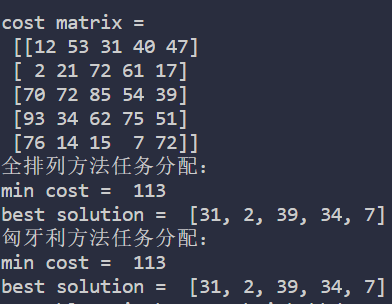
\includegraphics[scale=0.8]{找对象binary.png}\\
    \textit{图八:找对象算法结果(全排列和匈牙利算法)}
\end{center}
结果说明:\\
const matrix:常量矩阵,随机生成,$a_{ij}$代表i与j的边权值。\\
根据这个邻接矩阵,用全排列和匈牙利算法求得两种最小的权值cost。\\
并在best solution list中给出具体的边是哪一条。
\end{document}